% import packeges
\documentclass[a4paper,12pt]{article}
\usepackage[eng]{nbi}
\usepackage{paralist}
\usepackage[danish,english]{babel}
\usepackage[utf8]{inputenc}
\usepackage{graphicx}
\usepackage{geometry}
\usepackage{wrapfig}
\usepackage{eso-pic}
\usepackage{mathtools}
\usepackage{datetime}
\usepackage{nameref}
\usepackage{lastpage}
\usepackage{amsfonts}
\usepackage{appendix}
\usepackage{fancyheadings}
\usepackage{lipsum}
\usepackage{braket}

% definition environment
\usepackage{amsthm}
 
\theoremstyle{definition}
\newtheorem{definition}{Definition}[section]

\theoremstyle{theorem}
\newtheorem{theorem}{Theorem}[section]

% number equations by section
\numberwithin{equation}{section}

% set font type
\usepackage{times}

% redefinition of the plain style
\makeatletter
\newcommand*{\currentname}{\@currentlabelname}
\makeatother

% redefinition of the plain style
\fancypagestyle{plain}{
\lhead{Analysis of the BTZ Black Hole}
\rhead{\currentname}
\renewcommand{\footrulewidth}{0.5pt}
\cfoot{Page \thepage{} of 25}}

% create the front pages
\supervisor{Poul Henrik Damgaard and Subodh Patil}
\project{Bachelor project in physics}
\author{Christain Schiøtt and Rasmus Nielsen}
\title{Analysis of the BTZ Black Hole}
\subtitle{Properties of a (2+1) dimensional black hole solution}
\institute{Niels Bohr Institutet}
\department{Niels Bohr International Academy}
\email{bcn852@alumni.ku.dk and jbz701@alumni.ku.dk}
\handindate{13.06.2018}
\defencedate{To be decided}

\begin{document}

\maketitle

% The abstracts
% \newgeometry{top=4cm,left=4cm,right=4cm,bottom=4cm} 
%
\thispagestyle{empty}
%
%
\section*{Abstract}
We study various two-point functions in certain defect versions of $\mathcal{N} = 4$ super Yang Mills theory. These defect theories are obtained by insertion of a D7 probe-brane, with either $AdS_4 \times S^2 \times S^2$ or $AdS_4 \times S^4$ geometry, into the standard D3 brane configuration of AdS / CFT. The $\mathcal{N} = 4$ SYM theories, arising from the decoupling limit of these brane configurations, have non-zero vacuum expectation values (\textit{vevs}) for the scalar fields $\phi_i$. These non-zero vevs breaks super symmetry completely and conformal symmetry partially, thus presenting us with an interesting opportunity to make non-trivial tests of the AdS / CFT duality.\\
We focus first on two-point functions with $SO(3) \times SO(3)$ symmetric vevs, between chiral primary operators of the forms $\tr Z^L$, $\tr \bar{Z}^L$, $\tr X^L$, where $X = \phi_1 + i \phi_4$, $Y = \phi_2 + i \phi_5$ and $Z = \phi_3 + i \phi_6$. By use of pertubative methods, we were able to reduce the connected tree-level contributions to these two-point functions, down to expressions involving complicated infinite sums. These infinite sums unfortunately seem unevaluable in general. However, for specific values of $L$ and the parameters associated to stabilization of the brane configurations, we were able to explicitly evaluate the infinite sums.\\
We also study two-point functions, first with $SO(3) \times SO(3)$ symmetric vevs, between short scalar operators $\mathcal{O}_{W_1 W_2} = \tr[W_1 W_2]$ with scalars $W_1,W_2 = X,Y,Z, \bar{X}, \bar{Y}, \bar{Z}$, and Bethe state operators $\mathcal{O}_{L} = \Psi_M^{i_1 \ldots i_L} \tr[V_{i_1} \cdots V_{i_l}]$, with $V_i = X,Z$ and $\Psi_M$ being a Bethe wavefunction with $M$ excitations. By use of integrability techniques, we find that certain choices of $W_1,W_2$ allows for the tree-level contribution to these two-point functions to be expressed in terms of the tree-level value of $\expval{\mathcal{O}_{L}}$. The computations of these various types of two-point functions provide the first step towards a very non-trival check of the AdS / CFT duality. We hope that future work will enable us to complete this endeavor, by studying the corresponding objects on the gravity side of the duality. 

%The types of two-point functions subject to analysis are 1. two-point functions between scalar single-trace chiral primary operators, and 2. two-point functions between short single-trace scalar operators and Bethe state operators. By use of pertubative methods, we were able to reduce the tree-level contributions to the chiral primary two-point functions, down to infinite sums which generally seem uncomputable. For very specific parameter values associated to the operators and defect setups, we were able to evaluate the sums, and obtain explicit values for the tree-level contributions to these two-point functions.

\newpage
\thispagestyle{empty}
%
%
\section*{Acknowledgements}
I would like to thank my supervisor \textit{Charlotte Kristjansen}, first for presenting me with the opportunity to write this thesis, and subsequently for taking time to answer my seemingly endless stream of questions regarding the subject of this thesis, as well as AdS/CFT in general. I would also like to thank \textit{Matthias Wilhelm} and \textit{Matthias Volk} for engaging in many helpful discussions, as well as sharing thier valuable knowledge on the topic of this thesis. A big thank you also goes out to \textit{Marius de Leeuw}, who generously shared with me some very helpful Mathematica notebooks, concerning the computation of certain results from \cite{Two-point functions in D5-D3} relevant to this thesis. Similarly, I would also like to thank \textit{Isak Buhl-Mortensen} for his very helpful notes on the reduction of $10D$ Majorana-Weyl fermions to $4D$ Majorana fermions.\\
I would also like to thank my fellow master students for engaging in many stimulating discussions about our respective theses and physics in general. Particular gratitude goes out to \textit{Khalil Idiab}, with whom I have shared \textit{Charlotte Kristjansen} as supervisor. As the contents of our respective works were, and still is, closely connected, his input and suggestions have been of great value to me. Particular gratitude also goes out to \textit{Christian Schi\o tt}, who has been a dear friend to me throughout my time at university. Your help and advice has been invaluable.\\
In addition, I would like to thank my family; my mother in particular, the care and support of whom I am eternally grateful for. Lastly, I would like to thank my dear friend \textit{Peter Gross}. Without your help, this thesis would likely never have been brought to completion. Thank you. 
%
%

\newpage

% The table of contents
\tableofcontents
\thispagestyle{empty}
\setcounter{page}{0}

\newpage
\pagestyle{plain}

% section 1: Introduction
\newgeometry{top=2cm,left=2cm,right=2cm,bottom=2cm} 
%
\section{Introduction}
In this thesis, we set out to investigate the properties of the (2+1) dimensional black hole solution, discovered by \textbf{Máximo Bañados}, \textbf{Claudio Teitelboim}, and \textbf{Jorge Zanelli}, known as the \textbf{BTZ black hole}. Our aim is to first discuss the properties of the solution from the perspective of classical general relativity, of which a brief review is located in appendix A. Following that, we aim to investigate the consequences of having the BTZ spacetime be the background of a quantum scalar field theory. As will be shown, the BTZ Green's functions (sometimes referred to as two-point functions) will obey the KMS condition and the black hole will have a non-zero temperature, as is also the case for the Schwarzschild black hole. The structure of the thesis will be as follows:\newline
In \textbf{section 1}, we will first introduce the basic concepts of event horizons and black holes. We will then discuss the properties of some black hole solutions in (3+1) dimensions. Following that, some general features of quantum field theory in curved spaces are discussed. Lastly, we will go over the general features of standard general relativity in (2+1) dimensions.\newline
In \textbf{section 2}, we derive the BTZ metric by solving the \textbf{Einstein Equations} in (2+1) dimensions, assuming the existence of a time-like and a space-like \textbf{Killing vector}. We then discuss how the BTZ spacetime can be obtained by identifying certain points of the 3 dimensional \textbf{anti-de Sitter spacetime}.\newline
In \textbf{section 3}, we investigate the causal structure of the maximally extended static BTZ spacetime. We also discuss the nature of the singularities of the BTZ spacetime, and the existence of \textbf{closed time-like curves} under a specific extension of the spacetime.\newline
In \textbf{section 4}, we first discuss the \textbf{KMS condition} and how it implies that periodicity in imaginary time of the scalar field two-point functions give rise to a non-zero temperature. We then compute the two-point functions on $AdS_3$, and connect them to those of the static BTZ spacetime through the method of images. Lastly, we demonstrate that the static BTZ Green's functions obey the KMS condition, implying a non-zero temperature for the static BTZ black hole.
%
%
%As a final remark, we discuss how the observed temperature can also be obtained by analytic continuation of the static BTZ spacetime.
%
% Not anymore

\subsection{Black hole solutions}
%
The popular idea of a black hole is something all-devouring, something so massive that it is impossible to escape its gravitational pull. A physicists idea of a black hole is not too far from that image, but to give a proper definition of a black hole, we must first define the concept of an event horizon:
%
\theoremstyle{definition}
%
\begin{definition}{\textbf{Event Horizons:}}
The (\textit{future / past}) event horizon of an asymptotically maximally symmetric spacetime, is the boundary of the causal (\textit{past / future}) of conformal infinity $\mathcal{J}$. The causal (\textit{past / future}) of conformal infinity is denoted $J^{\pm}(\mathcal{J})$.
\end{definition}
%
%
\noindent
A \textbf{black hole} is then simply defined as $\mathcal{M} \setminus J^{-}(\mathcal{J})$, where $\mathcal{M}$ is the entire spacetime. This means that any future-directed timelike world line that goes into the black hole is unable to reach null infinity, which is what gives rise to the popular interpretation of black holes that a black hole is something you can not escape.
%
%
\subsubsection{The Schwarzschild Black Hole}
The simplest and most well-known black hole solution is the Schwarzschild black hole in (3+1)-dimensions, with the Schwarzschild metric written in Schwarzschild coordinates as:
%
%
\begin{equation}
ds^2 = -\bigg[1 - \frac{2 \, G \, M}{r} \bigg] \, \mathrm{d}t^2
+ \bigg[1 - \frac{2 \, G \, M}{r} \bigg]^{-1} \, \mathrm{d}r^2
+ r^2 \, \mathrm{d}\Omega_2^2
\end{equation}
%
\begin{equation}
t \in (-\infty, \infty)
\quad , \quad
r \in (0, 2 \, G \, M) \cup (2 \, G \, M, \infty)
\end{equation}
%
%
In the above metric, $d\Omega_2^2$ stands for the metric of a 2-sphere in the usual spherical coordinates. This metric has an apparent singularity at $r = 2 \, G \, M$, but a change of coordinates reveals that it is only a coordinate singularity. The only real singularity is at $r = 0$ where the curvature invariant $R_{\rho\sigma\mu\nu} \,R^{\rho\sigma\mu\nu} $ becomes infinite. One set of coordinates in which this can be seen is the Kruskal–Szekeres coordinates in which the metric takes the form:
%
%
\begin{equation}\label{SW_metric_kruskal}
ds^2 = \frac{32 \, G^3 \, M^3}{r} \, e^{r \, / \, 2 \, G \, M} \,
(-\mathrm{d}T^2 + \mathrm{d}X^2)
+ r^2 \, d\Omega_2^2
%
\quad , \quad
%
T^2 - X^2 < 1
\end{equation}
%
%
In the above $r$ is regarded as an implicit funtion of $X$ and $T$. Switching to these coordinates not only reveals the non-singular nature of the event horizon, it also reveals another curious fact about the spacetime: The traditional Schwarzschild coordinates do not cover the entire spacetime. When switching to Kruskal-Szekeres coordinates, it is possible to follow geodesics to extend the spacetime into a geodesically complete spacetime; a spacetime in which no geodesics stop at finite parameter value. Two diagrams are used to study the causal structure of this maximally extended spacetime; the \textbf{Kruskal diagram} and the \textbf{Conformal diagram}.
%
\begin{figure}[h!]
%
\centering
%
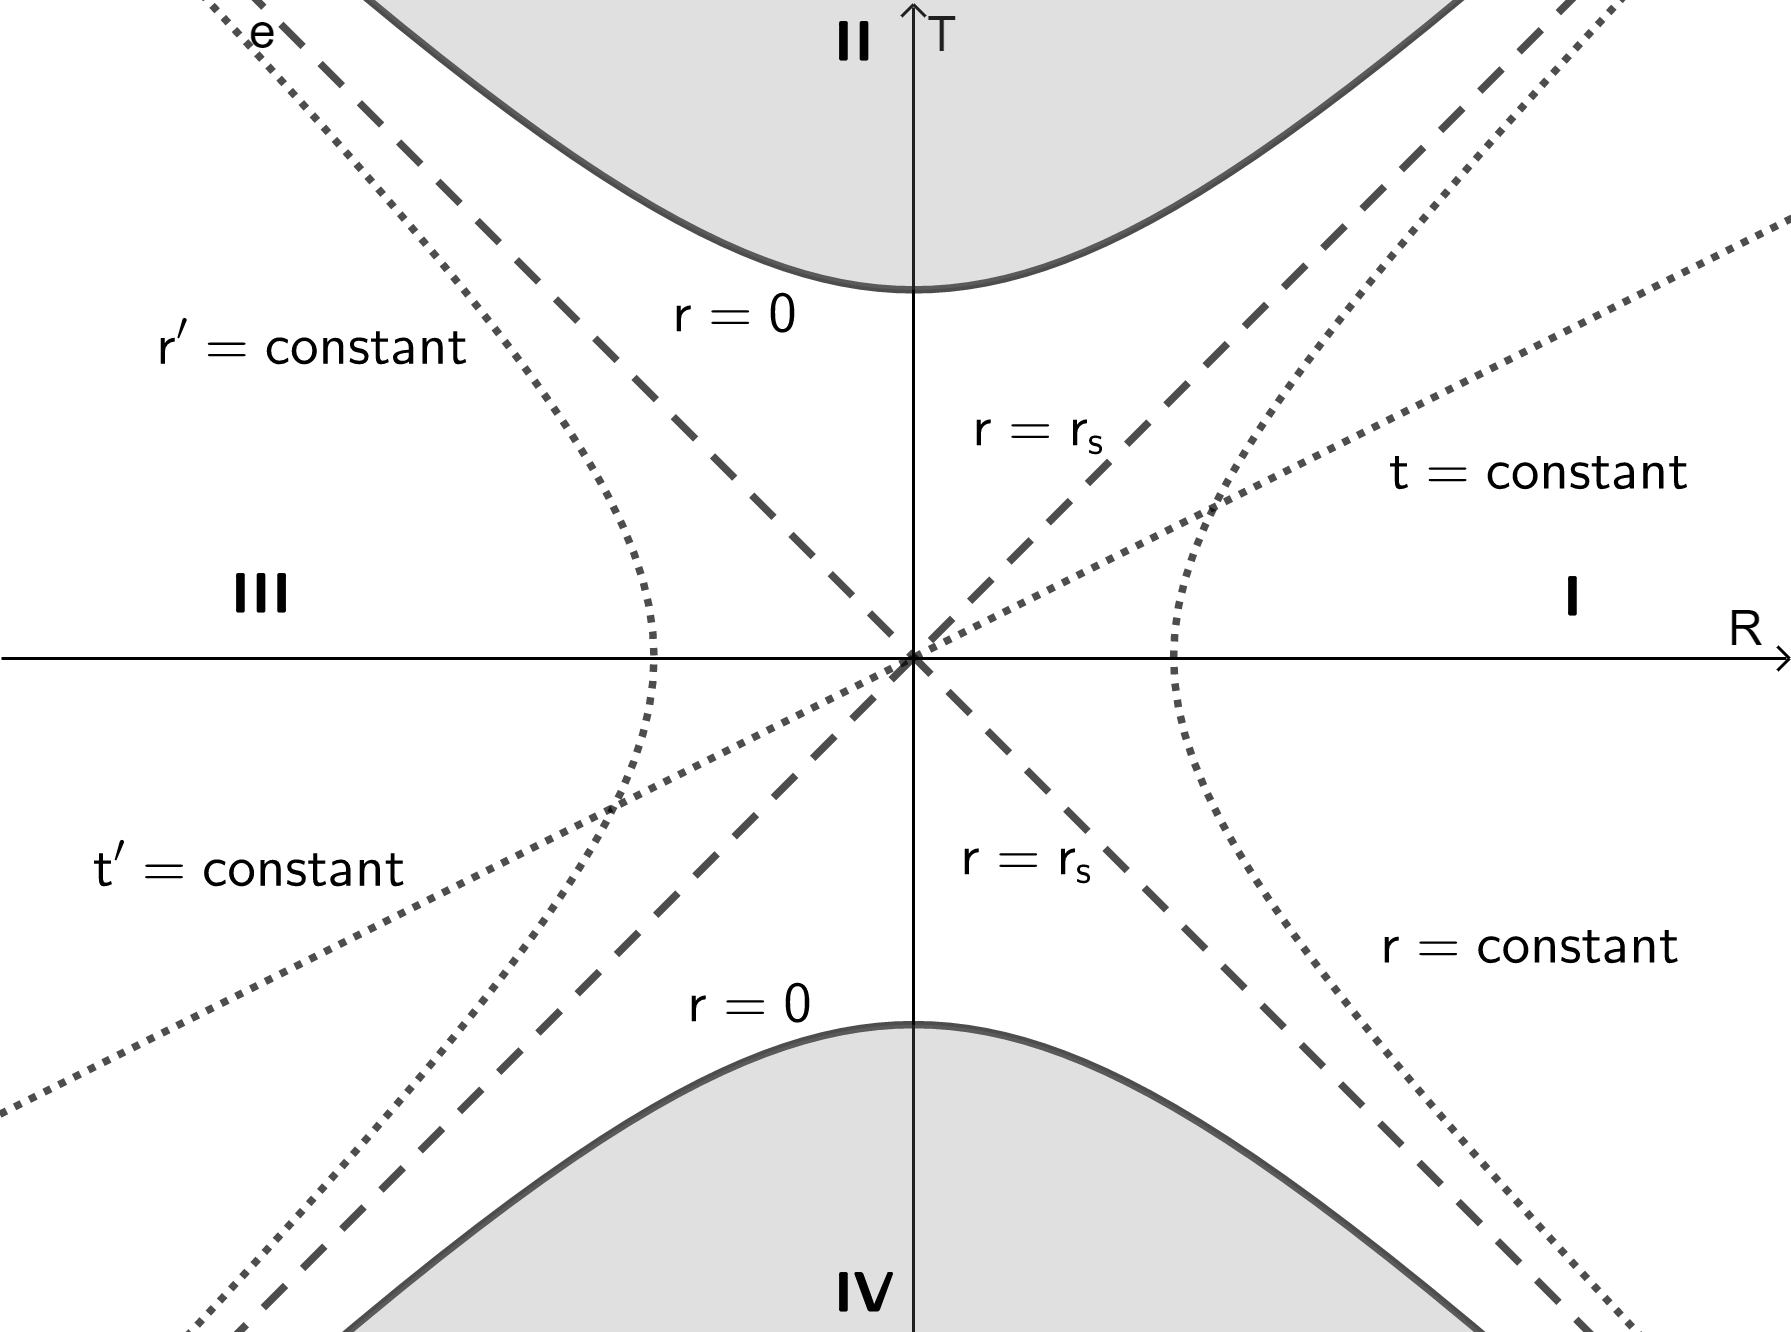
\includegraphics[width=0.69\textwidth]{../pics/Kruskal_Schwarz.png}
%
\caption{Kruskal diagram for the maximally extended Schwarzschild spacetime. The event horizon is located at $r=r_s$, while the curvature singularity is located at $r=0$. The grey areas above and below the $r = 0$ curves are not part of the spacetime.}
%
\label{fig:Kruskal_SW}
%
\end{figure}
%
\newline \noindent
The Kruskal diagram shows the spacetime in the Kruskal-Szekeres coordinates, where light cones stand upright and at $45^{\circ}$ everywhere, as can easily be seen from (\ref{SW_metric_kruskal}). The event horizon at $r = r_s$ naturally seperates the spacetime into four regions. The regions I and III are two disconnected (\textit{meaning not connected by future- or past-directed causal curves}) regions. The region II is the black hole, where hitting the singularity at $r = 0$ is unavoidable following any future-directed timelike path. The most surprising region IV, is called the white hole, and is the time-reversed version of the black hole. This means that all past-directed timelike paths in region IV, must hit the singularity at $r = 0$, or equivalently that it is impossible to enter the white hole from region I or III.\newline \newline
%
%
The Conformal diagram shows the spacetime in a set of compact coordinates, such that the nature of the infinities becomes more apparent. For example, we can easilly see that the structure of the conformal infinities in the regions I and III are identical to that of Minkowski space. We therefore call the Schwarzschild spacetime asymptotically flat. As in the Kruskal diagram, light cones stand upright and at $45^{\circ}$ everywhere in the Conformal diagram.
%
%
\begin{figure}[h!]
%
\centering
%
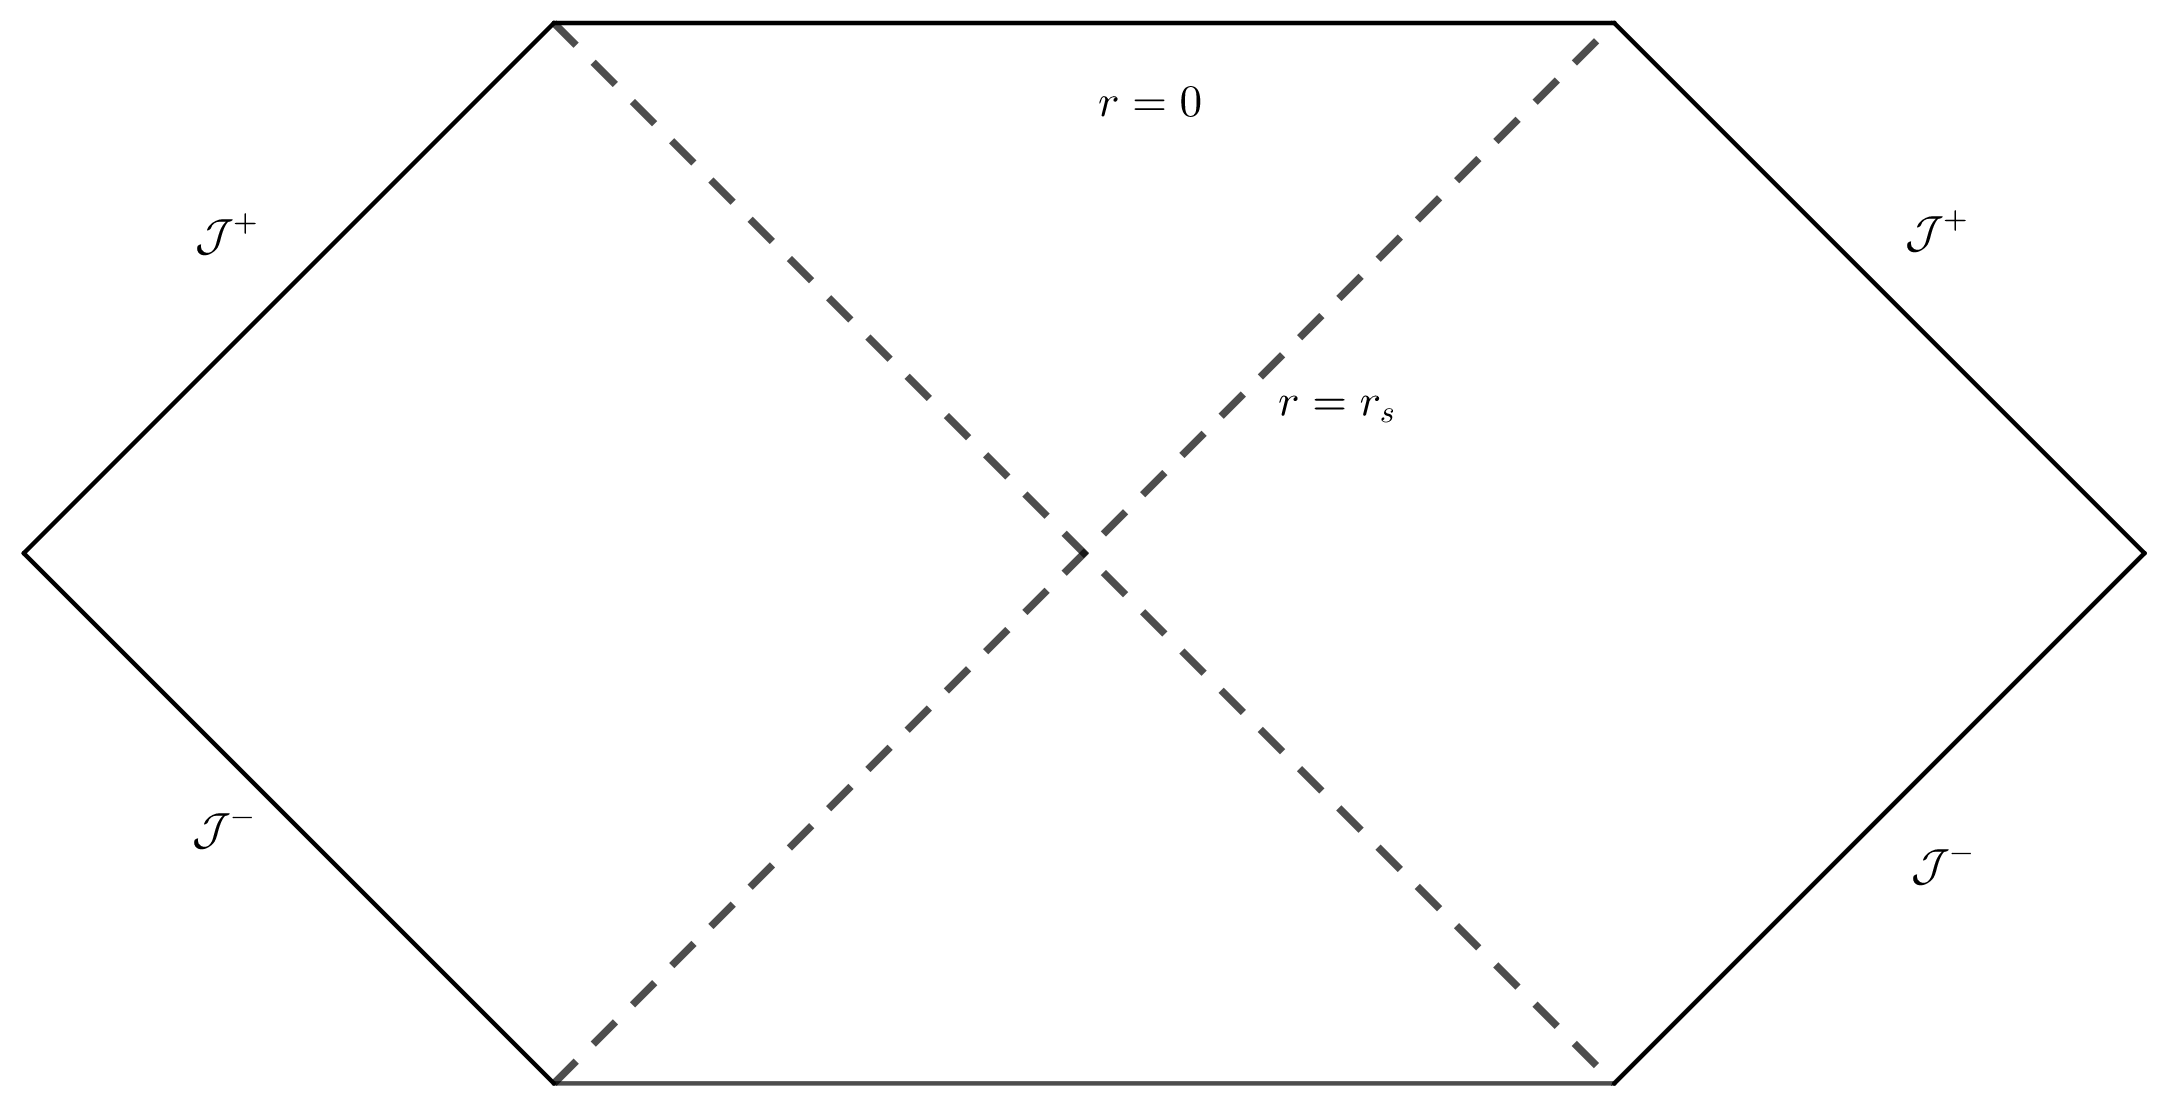
\includegraphics[width=0.86\textwidth]{../pics/SW_stat_Pen.png}
%
\caption{Conformal diagram for the maximally extended Schwarzschild spacetime. The future and past event horizons are located at $r=r_s$, while the curvature singularity is located at $r=0$. Past null infinity $\mathcal{J}^-$ is completely disjoint from future null infinity $\mathcal{J}^+$ in the two asymptotically flat regions.}
%
\label{fig:conformal_SW}
%
\end{figure}
%
%
%

\subsubsection{No-hair Theorem and the Information Paradox}
% Commented out for the time being
%
%%%%%%%%%%%%%%%%%%%%%%%%%%%%%%%%%%%%%%%%%%%%%%%%%%%%%%%%%%%%%%%%%%%%%%%%%%%%%%%%%%%%
%\textit{"Stationary, asymptotically flat black hole solutions to general relativity coupled to electromagnetism that are nonsingular outside the event horizon are fully characterized by the parameters of mass, electric and magnetic charge, and angular momentum."} [Carroll, page 238]\newline \newline
%%%%%%%%%%%%%%%%%%%%%%%%%%%%%%%%%%%%%%%%%%%%%%%%%%%%%%%%%%%%%%%%%%%%%%%%%%%%%%%%%%%%
%
%
Sean Carroll formulates a no-hair theorem in his book \textit{Spacetime and Geometry} in the following way:
%
\theoremstyle{theorem}
%
\begin{theorem}{\textbf{Black holes have no hair:}}
Stationary, asymptotically flat black hole solutions to general relativity coupled to electromagnetism, in 4 or less dimensions, that are nonsingular outside the event horizon, are fully characterized by the parameters of mass, electric and magnetic charge, and angular momentum. \cite{GR} %page 238
\end{theorem}
%
%
\noindent
The essence of this theorem and the reason for its name, is that there are only a small number of properties, parameterizing all black hole solutions. Namely, the mass, charge and spin of the spacetimes. These quantaties can be defined using for example the \textbf{Komar integrals}. This, together with phenomenon of \textbf{Hawking radiation} gives rise to the information paradox, that the information contained in matter seems to be lost when it passes the event horizon of a black hole.


\subsubsection{The Kerr Black Hole}
The Schwarschild Black Hole already discussed is a lot less hairy than what is required by the above no-hair theorem; both its spin and its charge is zero. An example of a Black Hole solution with a non-zero spin would be the \textbf{Kerr Black Hole}, which has a quite intricate metric given in \cite{GR}, which we will state in \textbf{Boyer-Lindquist coordinates} for completion:
%
%
\begin{align}\label{kerr_metric}
ds^2 = & - \left( 1 - \frac{2 \, G \, M \, r}{\rho^2} \right) \mathrm{d}t^2
- \frac{2 \, G \, M \, a \, r \, \sin^2\theta}{\rho^2}
(\mathrm{d}t \, \mathrm{d}\phi + \mathrm{d}\phi \, \mathrm{d}t) \notag\\
& + \frac{\rho^2}{\Delta}\mathrm{d}r^2
+ \rho^2 \, \mathrm{d}\theta^2
+ \frac{\sin^2\theta}{\rho^2} \left[
(r^2 + a^2)^2 - a^2 \Delta \sin^2{\theta}
\right] \mathrm{d}\phi^2
\end{align}
%
\begin{equation}
t \in (-\infty, \infty)
\quad , \quad
r \in (0, r_-) \cup (r_-, r_+) \cup (r_+, \infty)
\quad , \quad
\theta \in (0, \pi)
\quad , \quad
\phi \in (0, 2 \pi)
\end{equation}
%
%
The quantities $\Delta$ and $\rho$ are defined in terms of the coordinates and parameters as follow:
%
%
\begin{equation}
\Delta(r) = r^2 - 2 \, G \, M \, r + a^2
\end{equation}
%
\begin{equation}
\rho^2(r,\theta) = r^2 + a^2 \cos^2{\theta}
\end{equation}
%
%
%%%%%%%%%%%%%%%%%%%%%%%%%%%%%%%%%%%%%%%%%%%%%%%%%%%%%%%%%%%%%%%%%%%%%%%%%%%%%%%%%%%%%%%%
%The Kerr Black Hole has two event horizons: an outer horizon at $r=r_+$, and an inner horizon at $r=r_-$, which makes the causal structure a bit differently from that of the Schwarzschild Black Hole. A particle crossing the outer horizon is \textit{not} forced to pass the ringularity at $\rho = 0$, it is only forced to move towards the ringularity until it crosses the inner horizon. After crossing the inner horizon, the particle is free to move around, and even go through the ringularity, but if it crosses the inner horizon, it will be forced to move away from the ringularity until it crosses the outer horizon again. Furthermore, it will not return to the asymptotically flat region it came from, but rather to a new asymptotically flat region. This means that the area between the outer and inner horizon acts as a black hole (\textit{pulling everything in}), while the area between the inner and outer horizon acts as a black hole (\textit{pushing everything out}). The area past the inner horizon is sometimes called a \textbf{wormhole}. This all becomes more clear when looking at the Conformal diagram for the maximally extended Kerr spacetime.
%%%%%%%%%%%%%%%%%%%%%%%%%%%%%%%%%%%%%%%%%%%%%%%%%%%%%%%%%%%%%%%%%%%%%%%%%%%%%%%%%%%%%%%%
The \textbf{Komar mass} and \textbf{Komar angular momentum} of the Kerr balck hole are respectively $M$ and $M a$. The spacetime posses a curvature singularity at $\rho=0$, corresponding to $r=0$ and $\theta = \frac{\pi}{2}$. Unlike for the Schwarzschild black hole, the singularity is actually a ring and not a point. For this reason, It is referred to as a \textbf{ringularity}. The spacetime has two event horizons, an outer and an inner horizon, corresponding to the two values of $r$ for which $g^{rr} = 0$:
%
%
\begin{equation}
g^{rr}(r) = 0
\quad \Rightarrow \quad
r_{\pm} = G \, M \pm \sqrt{G^2 \, M^2 - a^2}
\end{equation}
%
%
We will later explain this method of identifying event horizons in more detail, when identify the horizons of the BTZ spacetime. In-between the inner and outer horizon, any future directed time-like curve is forced to move in the direction of decreasing $r$. In the region past the inner horizon, any time-like path is free to either go back through the inner horizon or go through the ringularity. The region past the ringularity is the extension of the spacetime to values of $r < 0$. It is sometimes referred to as the \textbf{anti universe}. It can easily be shown that the metric (\ref{kerr_metric}) restricted to curves of $t=const$, $r=const$ and $\theta = \frac{\pi}{2}$, with $r \ll 1$, become:
%
%
\begin{equation}
ds^2 \approx a^2 \, \left( 1 + \frac{2 \, G \, M}{r} \right) \mathrm{d}\phi^2
\end{equation}
%
%
Since $\phi \sim \phi + 2 \pi$, it is clear that for $r < 0$, the curves described above become \textbf{closed time-like curves}. If instead of going through the ringularity, a time-like curve goes back through the inner horizon, it will be forced to move in the direction of decreasing $r$ until it passes the outer horizon. Furthermore, it will not return to the asymptotically flat region it came from, but rather to a new asymptotically flat region. This all becomes more clear when looking at the Conformal diagram for the maximally extended Kerr spacetime:
%
\begin{figure}[h!]
%
\centering
%
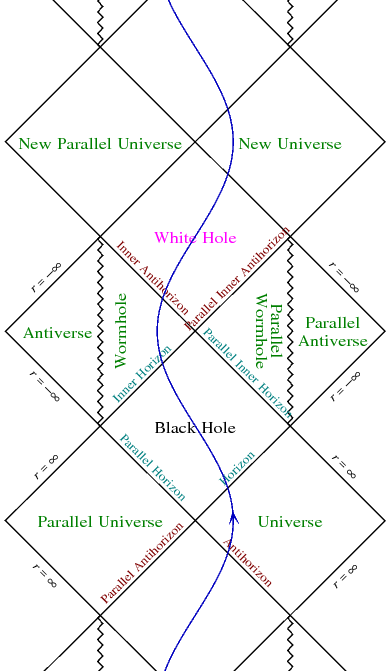
\includegraphics[width=0.38\textwidth]{../pics/penrose_kerr.png}
%
\caption{Conformal diagram for the Kerr spacetime. The blue line is the world line of a particle going through the wormhole. Found at https://jila.colorado.edu/~ajsh/insidebh/penrose.html}
%
\label{fig:conformal_SW}
%
\end{figure}


\subsection{Aspects of QFT on curved backgrounds}
In general curved spacetimes, the exist no notion of \textbf{global inertial coordinates}. As a consequence, there exists no preferred family of spacetime-foliations on which we can define a natural set of basis modes. Different sets of modes will be equally good and although they will exist in the same Hilbert space, they will define different Fock spaces, and specifically different vacuum states. A transformation between to sets of modes $f_i$ and $g_i$ is called a \textbf{Bogoliubov transformation} and given by \cite{GR}
%
%
\begin{equation}
g_i = \sum_j \left( \alpha_{i j} f_j + \beta_{i j} f_j^* \right) \quad , \quad
f_i = \sum_j \left( \alpha^*_{j i} g_j - \beta_{j i} g_j^* \right)
\end{equation}
%
%
The coefficients $\alpha_{i,j}$ and $\beta_{i,j}$ are called the Bogoliubov coefficients and also relate the annihilation and creation operators $\hat{b}_i, \hat{b}_i^{\dagger}$ for $g_i$ and $\hat{a}_i, \hat{a}_i^{\dagger}$ for $f_i$. 
%
%
\begin{equation}
\hat{a}_i = \sum_j \left( \alpha_{j i} \hat{b}_j + \beta_{j i}^* \hat{b}_j^{\dagger} \right) \quad , \quad
\hat{b}_i = \sum_j \left( \alpha^*_{i j} \hat{a}_j - \beta_{i j}^* \hat{a}_j^{\dagger} \right)
\end{equation}
%
%
We use this to calculate the expectation value of the number operator for $g$, $\hat{n}_{g i} = \hat{b}_{i}^{\dagger} \hat{b}_{i}$ in the vacuum state of $f$, $\ket{0_f}$.
%
%
\begin{equation}
\braket{0_f | \hat{n}_{g i} | 0_f} = \sum_{j} \beta_{i j} \beta_{i j}^* 
\end{equation}
%
%
And it now becomes apparent that what is a vacuum state for $f$ is observed in $g$ as a state containing particles.


\subsubsection{The Unruh Effect}
We will now briefly go through the simplest example of this difference in vacuum states, known as the Unruh effect, roughly following the structure of \cite{GR}. The Unruh effect can be stated as \\
\textit{"an accelerating observer in the traditional Minkowski vacuum state will observe a thermal spectrum of particles"} \cite{GR} \\
We start with ordinary (1+1)-dimensional Minkowski space and make the tranformation
%
\begin{equation}
x = \frac{1}{a} \, e^{a \xi} \, \sinh(a \eta) \quad, \quad
t = \frac{1}{a} \, e^{a \xi} \, \cosh(a \eta)
\end{equation}
%
We call the coordinates $(\xi, \eta)$ the \textbf{Rindler coordinates}. It can be shown that they cover the patch I given by $x>|t|$ known as \textbf{Rindler space} and that the we can cover the patch IV given by $x<|t|$ by simply adding a minus sign on each coordinate. In Rindler coordinates, curves of constant acceleration are given by
\begin{equation}
\eta(\tau) = \frac{\alpha}{a} \tau \quad, \quad
\xi(\tau) = \frac{1}{a} \ln \left( \frac{a}{\alpha} \right)
\end{equation}
and the metric takes the form
\begin{equation}
\mathrm{d}s^2 = e^{2 \alpha \xi} (- \mathrm{d} \eta^2 + \mathrm{d} \xi^2 )
\end{equation}
%
%
\begin{figure}[h!]
%
\centering
%
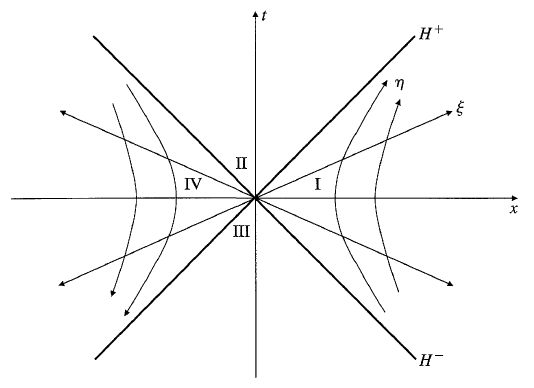
\includegraphics[width=0.8\textwidth]{../pics/Rindler_space.png}
%
\caption{A picture of flat space in Rindler coordinates. $H^+$ and $H^-$ are killing horizons of $\partial_{\eta}$. Found in \cite{GR}}
%
\end{figure}
%
%
Solving the Klein-Gordon equation $\Box \, \phi = 0$ in Rindler coordinates gives us plane waves, but because the future directed Killing vector is $\partial_{\eta}$ and $-\partial_{\eta}$ in patch I and IV respectively, we have a difference in sign for the positive frequency plane wave in the two regions, leading us to define two different plane wave solutions:
\begin{equation}
g_k^{(1)} = 
\begin{cases}
\frac{1}{\sqrt{4 \pi \omega}} e^{-i \omega \eta + i k \xi} & \text{I} \\
0 & \text{IV}
\end{cases}
\end{equation}
\begin{equation}
g_k^{(2)} = 
\begin{cases}
0 & \text{I} \\
\frac{1}{\sqrt{4 \pi \omega}} e^{i \omega \eta + i k \xi} & \text{IV}
\end{cases} \; \;
\end{equation}
We now have two different but equally good sets of modes in Rindler and Minkowski coordinates. We could in theory calculate the Bogoliubov coefficients for these modes and use that to evaluate the expectation value of the number operator for the Rindler coordinates in the Minkowski vacuum. However such a calculation would be long and cumbersome. In \cite{GR} this calculation has been made easier by introducing a set of modes that share the vacuum state with Minkowski but is simpler connected to the Rindler modes. We will not go through his calculation, but state his result:
\begin{equation}
\braket{0_M | \hat{n}_R^{(1)}(k) | 0_M} = \frac{1}{e^{2 \omega \pi / a} - 1} \delta(0)
\end{equation}
which is a thermal spectrum at the temp $T = \frac{a}{2 \pi}$. This is exactly the Unruh effect. A static observer at the event horizon of a Schwarzschild black hole will feel the gravitational pull of the black hole and therefore must be accelerated in order to stay at constant $r$. This leads \cite{GR} to explain Hawking Radiation in terms of the Unruh effect by noting that the spacetime is locally flat at the event horizon. This argument seems to hold for objects much less exotic than black holes though, since any static observer close to a gravitational body must accelerate to remain at a fixed distance to that body. A more convincing way to show that we can associate a temperature with the black hole is to show that its \textbf{Green's Function} has all the properties of a thermal Green's Function. We will show this explicitly in (2+1) dimensions, where Einstein gravity has some special properties.

%For that reason, we will instead argue for the Hawking Radiation by showing that the \textbf{Green's Function} for the BTZ black hole is periodic.



\subsection{Gravity in (2+1) dimensions}
One very important feature of standard Einstein gravity in (2+1) dimensions, is the fact that vacuum solutions have no local degrees of freedom. Said another way, all vacuum solutions to the \textbf{Einstein Equations} in (2+1) dimensions are locally isomorphic to one of the three maximally symmetric spaces; de Sitter space, ant-de Sitter space or Minkowski space. We will now show that this is indeed the case. Using the traces of the \textbf{Riemann tensor}; the \textbf{Ricci tensor} and \textbf{Ricci scalar}, we define a new tensor $C_{\rho\sigma\mu\nu}$, called the \textbf{Weyl tensor}. This tensor is defined by:
%
%
\begin{equation}\label{1.1}
C_{\rho\sigma\mu\nu} = R_{\rho\sigma\mu\nu}
- \frac{2}{(n-2)} \, (g_{\rho[\mu} \, R_{\nu]\sigma} - g_{\sigma[\mu} \, R_{\nu]\rho})
+ \frac{2}{(n-1) \, (n-2)} \, g_{\rho[\mu} \, g_{\nu]\sigma} \, R
\end{equation}
%
%
The Weyl tensor possesses the same symmetries as the Riemann tensor, and satisfies the condition:
%
%
\begin{equation}\label{1.2}
{C^{\rho}}_{\sigma\rho\nu} = 0
\end{equation}
%
%
Because the Weyl tensor and the Riemann tensor have the samme symmetries, the LHS of (\ref{1.2}) will be a symmetric tensor. It can be shown that the number of independent components of the Riemann tensor $D_{Riem}$, on an $n$-dimensional manifold is given by:
%
%
\begin{equation}
D_{Riem} = \frac{n^2 \, (n^2 - 1)}{12}
\end{equation}
%
%
The number of independent components of a symmetric $(0,2)$-tensor $D_{sym}$, on an $n$-dimensional manifold is of cause given by:
%
%
\begin{equation}
D_{sym} = \frac{n \, (n + 1)}{2}
\end{equation}
%
%
Thus, the number of independent components of the Wyel tensor $D_{Weyl}$, on an $n$-dimensional manifold will be given by:
%
%
\begin{equation}
D_{Weyl} = D_{Riem} - D_{sym} = \frac{n^2 \, (n^2 - 1)}{12} - \frac{n \, (n + 1)}{2}
\end{equation}
We see that for $n=3$, we have $D_{Weyl} = 0$. Thus, in a $3$-dimensional spacetime, we can use (\ref{1.1}) to express the Riemann tensor in terms of its traces:
%
%
\begin{equation}
R_{\rho\sigma\mu\nu} =
2 \, (g_{\rho[\mu} \, R_{\nu]\sigma} - g_{\sigma[\mu} \, R_{\nu]\rho})
- g_{\rho[\mu} \, g_{\nu]\sigma} \, R
\end{equation}
%
%
Now we look at the \textbf{Einstein Equations} in vacuum with a cosmological constant $\Lambda$:
%
%
\begin{equation}\label{1.7}
R_{\mu\nu} - \frac{1}{2} \, R \, g_{\mu\nu} + \Lambda \, g_{\mu\nu} = 0
\end{equation}
%
%
Taking the trace of (\ref{1.7}) we obtain, on a $3$-dimensional spacetime, the relation:
%
%
\begin{equation}\label{1.8}
R = 6 \, \Lambda
\end{equation}
%
%
If we now substitute (\ref{1.8}) back into (\ref{1.7}), we obtain the equation:
%
%
\begin{equation}
R_{\mu\nu} = 2 \, \Lambda \, g_{\mu\nu}
\end{equation}
%
%
Thus, for a metric on a $3$-dimensional spacetime, satisfying (\ref{1.7}), the Riemann tensor takes the form:
%
%
\begin{equation}
\boxed{
R_{\rho\sigma\mu\nu} =
\Lambda \, (g_{\rho\mu} \, g_{\nu\sigma} - g_{\rho\nu} \, g_{\mu\sigma})
}
\end{equation}
%
%
We now see that any solution to the Einstein equations, on a $3$-dimensional spacetime, will locally be isomorphic to a \textbf{maximally symmetric} space (\textit{$dS_3$, $AdS_3$ or $M_3$, depending on the sign of $\Lambda$}).

%%%%%%%%%%%%%%%%%%%%%%%%%%%%%%%%%%%%%%%%%%%%%%%%%%%%%%%%%%%%%%%%%%%%%%%%%%%%%%%%%%%%%%%
%From (\ref{1.8}), we also see that the \textbf{Einstein-Hilbert action}:
%%
%%
%\begin{equation}
%I_{EH} = \frac{1}{16 \, \pi \, G} \, \int_{\mathcal{M}} d^3x \, \sqrt{-g}  \, (R - 2 \, \Lambda)
%\end{equation}
%%
%%
%Will in general be infinte, for non-compact spacetime manifolds $\mathcal{M}$. Therefore, a boundary term is usually added to the Einstein-Hilbert action, such that the total action becomes:
%%
%%
%\begin{equation}
%I = \frac{1}{16 \, \pi \, G} \, \bigg[ 
%\int_{\mathcal{M}} d^3x \, \sqrt{-g}  \, (R - 2 \, \Lambda)
%+ \int_{\partial \mathcal{M}} d^2x \, \sqrt{-h} \, K
%\bigg]
%\end{equation}
%%
%%
%Where $h_{ij}$ is the induced metric on $\partial \mathrm{M}$, and $K_{ij}$ is the extrinsic curvature on $\partial \mathrm{M}$.
%%%%%%%%%%%%%%%%%%%%%%%%%%%%%%%%%%%%%%%%%%%%%%%%%%%%%%%%%%%%%%%%%%%%%%%%%%%%%%%%%%%%%%%


% section 2: The Metric
\newgeometry{top=2cm,left=2cm,right=2cm,bottom=2cm} 
%
\section{Derivation of the BTZ metric}
As we proved in the last section, all vacuum solutions to the \textbf{Einstein Equations} in (2+1) dimensions are locally isomorphic to either de Sitter space, anti-de Sitter space or Minkowski space. Thus, all the information about any particular solution will be contained in its topology. Despite this, it is still very worthwhile to derive the BTZ metric in what we will call \textbf{Schwarzschild-like coordinates}, under the assumptions of stationarity and circular symmetry. There are several reasons for this, some of which being: it is easy to identify event horizons, the mass and angular momentum parameters will stand out clearly and the description of the spacetime in terms of identifying points in $AdS_3$ will be particularly simple. With all that said, let us begin the derivation.

\subsection{An ansatz for the Einstein Equations}
On a $3$-dimensional spacetime, a general metric tensor will have $3 \, (3 + 1) / 2 = 6$ independent components, $3$ of which can be arbitrarily changed by coordinate transformations. We will use this freedom to assume the following form of the metric: 
%
%
\begin{equation}\label{2.1}
ds^2 = -f^2(t,r,\phi) \, \mathrm{d}t^2
+ g^2(t,r,\phi) \, \mathrm{d}r^2
+ r^2 \, [\mathrm{d}\phi - h(t,r,\phi) \, \mathrm{d}t]^2
\end{equation}
%
%
We will discuss the ranges of these coordinates when the metric is fully derived. We assume of (\ref{2.1}) that it be both stationary and circularly symmetric. This corresponds to the metric possessing two \textbf{Killing vectors}: $R = \partial_{\phi}$, $K = \partial_t$. In order for (\ref{2.1}) to be invariant under the flow of $R$ and $K$, the metric must satisfy the conditions:
%
%
\begin{align}\label{2.2}
\mathcal{L}_{R} \, g_{\mu \nu} & =
R^{\lambda} \, \frac{\partial g_{\mu \nu}}{\partial x^{\lambda}}
+ g_{\lambda \nu} \, \frac{\partial R^{\lambda}}{\partial x^{\mu}}
+ g_{\mu \lambda} \, \frac{\partial R^{\lambda}}{\partial x^{\nu}} =
\frac{\partial g_{\mu \nu}}{\partial \phi} = 0
\notag\\
\mathcal{L}_{K} \, g_{\mu \nu} & =
K^{\lambda} \, \frac{\partial g_{\mu \nu}}{\partial x^{\lambda}}
+ g_{\lambda \nu} \, \frac{\partial K^{\lambda}}{\partial x^{\mu}}
+ g_{\mu \lambda} \, \frac{\partial K^{\lambda}}{\partial x^{\nu}} =
\frac{\partial g_{\mu \nu}}{\partial t} = 0
\end{align}
%
%
Where $\mathcal{L}_{X}$ is the \textbf{Lie derivative} in the direction of the vector $X$. The conditions (\ref{2.2}) simply implies that the components of the metric be independent of $\phi$ and $t$. We can thus write the metric (\ref{2.1}), our ansatz for the Einstein Equations, in the form:
%
%
\begin{equation}\label{2.3}
ds^2 = -f^2(r) \, \mathrm{d}t^2
+ g^2(r) \, \mathrm{d}r^2
+ r^2 \, [\mathrm{d}\phi - h(r) \, \mathrm{d}t]^2
\end{equation}
%
%


\subsection{Solving the Einstein Equations}
In section 1.3 on Einstein gravity in (2+1) dimensions, we found that the vacuum \textbf{Einstein equations} on a $3$-dimensional spacetime, could be brought to the following form:
%
%
\begin{equation}\label{2.7}
R_{ij} = 2 \, \Lambda \, g_{ij}
\end{equation}
%
%
In order to find solutions to (\ref{2.7}), we first compute the \textbf{Ricci tensor} $R_{ij}$. We will do this using the \textbf{orthonormal frame method}, also sometimes called the triad method. We start by constructing an orthonormal basis of 1-forms $\epsilon^i$:
%
%
\begin{equation}
\epsilon^0 = f(r) \, \mathrm{d}t
\quad , \quad
\epsilon^1 = g(r) \, \mathrm{d}r
\quad , \quad
\epsilon^2 = r \, [\mathrm{d}\phi
- h(r) \, \mathrm{d}t]
\end{equation}
%
%
In the basis of the orthonormal 1-forms $\epsilon^i$, the metric manifestly becomes diagonal, meaning that:
%
%
\begin{equation}
ds^2 = \eta_{ij} \, \epsilon^i \otimes \epsilon^j
= -\epsilon^0 \otimes \epsilon^0
+ \epsilon^1 \otimes \epsilon^1
+ \epsilon^2 \otimes \epsilon^2
\end{equation}
We can now employ the orthonormal 1-form basis $\epsilon^i$ to find the \textbf{connection 1-forms} ${\omega^i}_j$, using the first \textbf{Cartan structure equation}:
%
%
\begin{equation}\label{2.9}
\Theta^i = \mathrm{d}\epsilon^i + {\omega^i}_j \wedge \epsilon^j = 0
\end{equation}
%
%
The components $g_{ij}$ are the metric components with respect to the basis $\epsilon^i$, and $\Theta^i$ are the \textbf{torsion 2-forms}. The requirement that our connect be torsion-free and metric compatible, impose the following requirements on $\Theta^i$ and ${\omega^i}_j$:
%
%
\begin{equation}\label{reqs}
\Theta^i = 0
\quad , \quad
\omega_{ij} = -\omega_{ji}
\quad , \quad
\omega_{ij} := g_{ik} \, {\omega^k}_j
\end{equation}
%
%
We now look for solutions to (\ref{2.9}) satisfying the requirements (\ref{reqs}). We start by computing the exterior derivative of our basis 1-forms $\epsilon^i$:
\begin{equation}
\mathrm{d}\epsilon^0 = F(r) \, \epsilon^1 \wedge \epsilon^0
\quad , \quad
\mathrm{d}\epsilon^1 = 0
\quad , \quad
\mathrm{d}\epsilon^2 = G(r) \, \epsilon^1 \wedge \epsilon^2
- H(r) \, \epsilon^1 \wedge \epsilon^0
\end{equation}
%
%
Here, the functions $F(r)$, $G(r)$ and $H(r)$, are given in terms of $f(r)$, $g(r)$ and $h(r)$ by:
%
%
\begin{equation}\label{2.11}
F(r) := \frac{f'(r)}{f(r) \, g(r)}
\quad , \quad
G(r) := \frac{1}{r \, g(r)}
\quad , \quad
H(r) := \frac{r \, h'(r)}{f(r) \, g(r)}
\end{equation}
%
%
The structure equation (\ref{2.9}) with restrictions (\ref{reqs}) in our orthonormal basis $\epsilon^i$ then becomes:
%
%
\begin{align}
F(r) \, \epsilon^1 \wedge \epsilon^0
+ {\omega^0}_1 \wedge \epsilon^1
+ {\omega^0}_2 \wedge \epsilon^2 & = 0
\notag\\
{\omega^1}_0 \wedge \epsilon^0
+ {\omega^1}_2 \wedge \epsilon^2 & = 0
\notag\\
G(r) \, \epsilon^1 \wedge \epsilon^2
- H(r) \, \epsilon^1 \wedge \epsilon^0
+ {\omega^2}_0 \wedge \epsilon^0
+ {\omega^2}_1 \wedge \epsilon^1 & = 0
\end{align}
%
Upon inspection, one finds that the following is a set of solutions to the above equations:
%
%
\begin{equation}
{\omega^0}_1 = F(r) \, \epsilon^0 - \frac{1}{2} \, H(r) \, \epsilon^2
\quad , \quad
{\omega^2}_1 = G(r) \, \epsilon^2 - \frac{1}{2} \, H(r) \, \epsilon^0
\quad , \quad
{\omega^2}_0 = \frac{1}{2} \, H(r) \, \epsilon^1
\end{equation}
%
%
We can now use the second \textbf{Cartan structure equation} to compute the \textbf{curvature 2-forms}:
%
%
\begin{equation}\label{2.10}
{\Omega^i}_j = \mathrm{d}{\omega^i}_j + {\omega^i}_k \wedge {\omega^k}_j
\end{equation}
%
%
We begin by computing the exterior derivative of each connection 1-form. The result is the following:
%
%
\begin{align}
\mathrm{d}{\omega^0}_1 & = \bigg[ \frac{F'(r)}{g(r)}
+ F^2(r)
- \frac{H^2(r)}{2} \bigg] \, \epsilon^1 \wedge \epsilon^0
%
+ \bigg[ \frac{H'(r)}{2 \, g(r)}
+ \frac{H(r) \, G(r)}{2} \bigg] \, \epsilon^1 \wedge \epsilon^2
\notag\\
\mathrm{d}{\omega^2}_1 & = \bigg[ \frac{G'(r)}{g(r)}
+ G^2(r) \bigg] \, \epsilon^1 \wedge \epsilon^2
%
- \bigg[ G(r) \, H(r)
+ \frac{H'(r)}{2 \, g(r)}
+ \frac{H(r) \, F(r)}{2} \bigg] \, \epsilon^1 \wedge \epsilon^0
\notag\\
\mathrm{d}{\omega^2}_0 & = 0
\end{align}
%
%
We now compute the wedge products between the connection 1-forms. The result is the following:
%
%
\begin{align}\label{struct_2_1}
{\omega^0}_2 \wedge {\omega^2}_1 & = \frac{H(r) \, G(r)}{2} \, \epsilon^1 \wedge \epsilon^2
- \frac{H^2(r)}{4} \, \epsilon^1 \wedge \epsilon^0
\notag\\
{\omega^2}_0 \wedge {\omega^0}_1 & = \frac{H(r) \, F(r)}{2} \, \epsilon^1 \wedge \epsilon^0
+ \frac{H^2(r)}{4} \, \epsilon^1 \wedge \epsilon^2
\notag\\
{\omega^2}_1 \wedge {\omega^1}_0 & = -\bigg[ G(r) \, F(r)
+ \frac{H^2(r)}{4} \bigg] \, \epsilon^0 \wedge \epsilon^2
\end{align}
%
%
Usings the results (\ref{struct_2_1}) and (\ref{struct_2_2}), we see that the second Cartan structure equation (\ref{2.10}) reads:
%
%
\begin{align}\label{struct_2_2}
{\Omega^0}_1 & = \bigg[ \frac{F'(r)}{g(r)}
+ F^2(r)
- \frac{3 \, H^2(r)}{4} \bigg] \, \epsilon^1 \wedge \epsilon^0
%
+ \bigg[ \frac{H'(r)}{2 \, g(r)}
+ H(r) \, G(r) \bigg] \, \epsilon^1 \wedge \epsilon^2
\notag\\
{\Omega^2}_1 & = \bigg[ \frac{G'(r)}{g(r)}
+ G^2(r)
+ \frac{H^2(r)}{4} \bigg] \, \epsilon^1 \wedge \epsilon^2
%
- \bigg[ G(r) \, H(r)
+ \frac{H'(r)}{2 \, g(r)} \bigg] \, \epsilon^1 \wedge \epsilon^0
\notag\\
{\Omega^2}_0 & = -\bigg[ G(r) \, F(r)
+ \frac{H^2(r)}{4} \bigg] \, \epsilon^0 \wedge \epsilon^2
\end{align}
%
%
The curvature 2-forms are related to the \textbf{Riemann tensor} components ${R^i}_{jkl}$, in the following way:
%
%
\begin{equation}
{\Omega^i}_j = \frac{1}{2} \, {R^i}_{jkl} \, \epsilon^k \wedge \epsilon^l
\end{equation}
%
%
The non-zero components (\textit{excluding those related by symmetry}) of the Riemann tensor are thus:
%
%
\begin{align}\label{2.14}
{R^0}_{110} & = \frac{F'(r)}{g(r)} + F^2(r) - \frac{3 \, H^2(r)}{4}
\notag\\
{R^0}_{112} & = \frac{H'(r)}{2 \, g(r)} + H(r) \, G(r)
\notag\\
{R^2}_{112} & = \frac{G'(r)}{g(r)} + G^2(r) + \frac{H^2(r)}{4}
\notag\\
{R^2}_{002} & = -G(r) \, F(r) - \frac{H^2(r)}{4}
\end{align}
%
%
From the above components of the Riemann tensor, we can now construct the non-zero components (\textit{excluding those related by symmetry}) of the \textbf{Ricci tensor} $R_{jl} := {R^i}_{jil}$. The result is the following:
%
%
\begin{align}
R_{00} & = \frac{F'(r)}{g(r)} + F^2(r) - \frac{H^2(r)}{2}
+ G(r) \, F(r)
\notag\\
R_{02} & = \frac{H'(r)}{g(r)} + 2 \, H(r) \, G(r)
\notag\\
R_{11} & = -\frac{F'(r)}{g(r)} - F^2(r) + \frac{H^2(r)}{2}
- \frac{G'(r)}{g(r)} - G^2(r)
\notag\\
R_{22} & = -\frac{G'(r)}{g(r)} - G^2(r) - \frac{H^2(r)}{2}
- G(r) \, F(r)
\end{align}
%
%
We are now ready to solve the vacuum Einstein Equations (\ref{2.7}). The $02$-component of the Einstein Equations immediately let us solve for the function $H(r)$:
%
%
\begin{equation}
R_{02} = 0
\quad \Rightarrow \quad
r \, H'(r) + 2 \, H(r) = 0
\quad \Rightarrow \quad
H(r) = -\frac{J}{r^2}
\end{equation}
%
%
Where $J \in \mathbb{R}$. As the name suggests, the integration constant $J$ is indeed the angular momentum of the spacetime. A discussion of this can be found in \cite{2+1 black hole}. In order to find the function $G(r)$, it is convenient to consider the following sum of Ricci components:
%
%
\begin{equation}
2 \, \Lambda = R_{00} + R_{11} + R_{22} = - 2 r \, \, G'(r) \, G(r)
- 2 \, G^2(r)
- \frac{H^2(r)}{2}
\end{equation}
%
%
If we now define a new function: $\Gamma(r) = r \, G(r)$, we get the following first order equation for $\Gamma(r)$:
%
%
\begin{equation}
2 \, \Gamma'(r) \, \Gamma(r)
+ \frac{r \, H^2(r)}{2}
= - 2 \, r \, \Lambda
\quad \Rightarrow \quad
\Gamma^2(r) = -M - \Lambda \, r^2 + \frac{J^2}{4 \, r^2}
\end{equation}
%
%
Where $M \in \mathbb{R}$. Again, as the name suggests, the integration constant $M$ turns out to be the mass of the spacetime. As with $J$, a discussion of this can be found in \cite{2+1 black hole}. If we compare the above result with the relations (\ref{2.11}), we see that:
%
%
\begin{equation}
g^{-2}(r) = r^2 \, G^2(r) = \Gamma^2(r)
\quad \Rightarrow \quad
g^{-2}(r) = -M - \Lambda \, r^2 + \frac{J^2}{4 \, r^2}
\end{equation}
%
%
In order to find the function $f(r)$, it is convenient to consider the following sum of Ricci components:
%
%
\begin{equation}\label{2.12}
0 = R_{00} + R_{11} = - G(r) \, \Gamma'(r) + G(r) \, F(r)
\quad \Rightarrow \quad
\frac{F(r)}{\Gamma(r)} = \frac{\Gamma'(r)}{\Gamma(r)}
\end{equation}
%
%
From the above equation (\ref{2.11}) and (\ref{2.12}), we find the following relation between $f(r)$ and $g(r)$:
%
%
\begin{equation}\label{2.13}
\frac{F(r)}{\Gamma(r)} = \frac{f'(r)}{f(r)}
\quad \Rightarrow \quad
\frac{\Gamma'(r)}{\Gamma(r)} = \frac{f'(r)}{f(r)}
\quad \Rightarrow \quad
k^2 \, g^{-2}(r) = f^2(r)
\end{equation}
%
%
Where $k \in \mathbb{R}$. Lastly, we get from (\ref{2.11}) and (\ref{2.13}) the following first order equation for $h(r)$:
%
%
\begin{equation}
h'(r) = \frac{k \, H(r)}{r} = -\frac{k \, J}{r^3}
\quad \Rightarrow \quad
h(r) = \frac{k \, J}{2 \, r^2} + c
\end{equation}
%
%
Where $c \in \mathbb{R}$. The integration constans $k$ and $c$ can be removed from the solution, by performing the following simple coordinate transforation:
%
%
\begin{equation}
\phi \to \phi - c \, t
\quad , \quad
t \to k \, t
\end{equation}
%
%
Thus, the final form of the metric (\ref{2.3}) becomes:
%
%
\begin{equation}\label{btz_metric}
\boxed{
ds^2 = -\bigg[-M - \Lambda \, r^2 + \frac{J^2}{4 \, r^2} \bigg] \, \mathrm{d}t^2
+ \bigg[-M - \Lambda \, r^2 + \frac{J^2}{4 \, r^2} \bigg]^{-1} \, \mathrm{d}r^2
+ r^2 \, \bigg[ \mathrm{d}\phi
- \frac{J}{2 \, r^2} \, \mathrm{d}t \bigg]^2
}
\end{equation}
When $\Lambda < 0$, this metric behaves like a black hole metric, and is called the \textbf{BTZ black hole} metric. To see that $\Lambda < 0$ is necessary for (\ref{btz_metric}) to be a black hole, one option is to investigate how the causal type (\textit{time-like, space-like or null}) of constant $r$ hypersurfaces changes with $r$. For black holes, we expect to see at least one value of $r$ for which the associated hypersurface is null, and we expect the hypersurfaces to be time-like for $r \to \infty$. In the coordinates $(t, r, \phi)$, the normal vectors of constant $r$ hypersurfaces $n^{\mu} = g^{\mu\nu} \, (\partial_{\nu}r)$, have the following metric norms:
%
%
\begin{equation}
g_{\mu\nu} \, n^{\mu} \, n^{\mu}
= g_{\mu\nu} \, g^{\mu\rho} \, (\partial_{\rho}r) \, g^{\nu\sigma} \, (\partial_{\sigma}r)
= g^{rr}(r)
\end{equation}
%
%
Thus, the values of $r^2$ for which the constant $r$ hypersurfaces become null are the following:
%
%
\begin{align}\label{null_values}
\Lambda \neq 0
\quad & : \quad
g^{rr}(r) = 0
\quad \Rightarrow \quad
r^2_{\pm}
=  -\frac{1}{2 \, \Lambda} \, \big[
M \pm \sqrt{M^2 + \Lambda \, J^2}
\big]
%
\notag\\
%
\Lambda = 0
\quad & : \quad
g^{rr}(r) = 0
\quad \Rightarrow \quad
r^2_+ = \frac{J^2}{4 \, M}
\end{align}
%
%
The number of solutions to the above equations depend on the sign of the cosmological constant $\Lambda$, and so does the sign of $g^{rr}(r)$ as $r$ varies, which determines the causal type of the hypersurfaces:
%
%
\begin{enumerate}
%
\item[$\Lambda > 0$:] there will be 0 or 1 solutions to (\ref{null_values}) with $r^2 > 0$, and $g^{rr}(r) < 0$ as $r \to \infty$.
%
\item[$\Lambda = 0$:] there will be 0 or 1 solutions to (\ref{null_values}) with $r^2 > 0$, and $g^{rr}(r) < 0$ as $r \to \infty$.
%
\item[$\Lambda < 0$:] there will be 0, 1 or 2 solutions to (\ref{null_values}) with $r^2 > 0$, and $g^{rr}(r) > 0$ as $r \to \infty$.
%
\end{enumerate}
%
%
The crucial point here, is that only for $\Lambda < 0$, constant $r$ hypersurfaces will be time-like at infinity. Thus, the BTZ spacetime will have the causal structure of a black hole only when $\Lambda < 0$. In the non-degenerate case, the spacetime will possess an outer and an inner event horizon, just as the (3+1) dimensional \textbf{Kerr black hole}. Thus, the ranges of the coordinates $(t, r, \phi)$ are:
\begin{equation}
t \in (-\infty, \infty)
\quad , \quad
r \in (0, r_-) \cup (r_-, r_+) \cup (r_+, \infty)
\quad , \quad
\phi \in (0, 2 \pi)
\end{equation}
%
%
The BTZ black hole has many other properties similar to those of black hole solutions in (3+1) dimensions, in particular the Kerr black hole. We will further explore these similarities, and important differences, in section 3.

\subsection{Connection to anti-de Sitter space}
Now that we have established that the BTZ metric is only describes a black hole spacetime when $\Lambda < 0$, we can begin to investigate how this affects the structure of the BTZ spacetime. From our discussion of Einstein gravity in (2+1) (\textit{section 1.3}) we know that $\Lambda < 0$ implies that the BTZ spacetime be locally isomorphic to 3 dimensional anti-de Sitter space, $AdS_3$. This means that we can potentially learn a lot about the BTZ spacetime by studying $AdS_3$, and we will now proceed to do so.

\subsubsection{Anti-de Sitter space}
One way of defining $AdS_3$ is by introducing an ambient $\mathbb{R}^4$ space, equipped with the following metric:
%
% 
\begin{equation}\label{ambient_metric}
dS^2
= \eta_{ab}^{(2,2)} \, \mathrm{d}X^a \, \mathrm{d}X^b
= -(\mathrm{d}X^0)^2 - (\mathrm{d}X^1)^2 + (\mathrm{d}X^2)^2 + (\mathrm{d}X^3)^2
\end{equation}
%
%
$AdS_3$ is then defined as a hypersurface in the ambient $\mathbb{R}^4$ space, through the following constraint:
%
%
\begin{equation}\label{anti-de sitter}
\eta_{ab}^{(2,2)} \, X^a \, X^b
= -(X^0)^2 - (X^1)^2 + (X^2)^2 + (X^3)^2
= -\ell^2
\end{equation}
%
%
We can now parametrize the points in $\mathbb{R}^4$ satisfying (\ref{anti-de sitter}), with the coordinates $(\lambda, \rho, \theta)$ as follow:
%
%
\begin{align}
X^0 = \ell \, \sin\lambda \, \cosh\rho
\quad & , \quad
X^1 = \ell \, \cos\lambda \, \cosh\rho
%
\notag\\
%
X^2 = \ell \, \sin\theta \, \sinh\rho
\quad & , \quad
X^3 = \ell \, \cos\theta \, \sinh\rho \label{ads_parameterized}
\end{align}
%
\begin{equation*}
\lambda \in (-\infty, \infty)
\quad , \quad
\rho \in (0, \infty)
\quad , \quad
\theta \in (0, 2 \pi)
\end{equation*}
%
%
The \textbf{pull-back} of the ambient metric (\ref{ambient_metric}) onto the $AdS_3$ hypersurface (\ref{anti-de sitter}), is then given by:
%
%
\begin{equation}\label{ads_metric}
ds^2 = g_{\mu\nu} \, \mathrm{d}x^\mu \, \mathrm{d}x^\nu
= \ell^2 \left(
-\cosh^2\rho \, \mathrm{d}\lambda^2
+ \mathrm{d}\rho^2
+ \sinh^2\rho \, \mathrm{d}\theta^2
\right)
\end{equation}
%
%
It should be noted that because we have chosen for $\lambda \in (-\infty, \infty)$, what we have constructed is technically the universal covering space of $AdS_3$, sometimes denoted by $\widetilde{AdS_3}$. we have done this to avoid the emergence of \textbf{closed time-like curves}, normally associated with the construction of $AdS_3$ as the hypersurface (\ref{anti-de sitter}). The Ricci tensor $R_{\mu\nu}$ and Ricci scalar $R$ can now be computed from the metric (\ref{ads_metric}). It can easily be checked that $R_{\mu\nu} = -2 \, \ell^{-2} \, g_{\mu\nu}$ and $R = - 6 \, \ell^{-2}$, confirming that $AdS_3$ is the constant negative curvature solution to the vacuum Einstein Equations with $\Lambda = -\ell^{-2}$.\newline
To investigate the causal structure of $AdS_3$ it is, as always, useful to construct a conformal diagram of the spacetime. In order to so, we perform the following coordinate transformation of the radial coordinate $\rho$:
%
%
\begin{equation}
\cosh\rho = \frac{1}{\cos\chi}
\quad \Rightarrow \quad
ds^2 = \frac{\ell^2}{\cos^2\chi} \, \left(
- \mathrm{d}\lambda^2
+ \mathrm{d}\chi^2
+ \sin^2\chi \, \mathrm{d}\theta^2
\right)
\end{equation}
%
%
From the above relation between $\rho$ and $\chi$, we can clearly see that $\chi \in \left( 0, \frac{\pi}{2} \right)$. $AdS_3$ is therefore conformally equivalent to an infinite strip if width $\frac{\pi}{2}$, as can be seen in the conformal diagram below:
%
\newpage
%
%
\begin{figure}[h!]
%
\centering
%
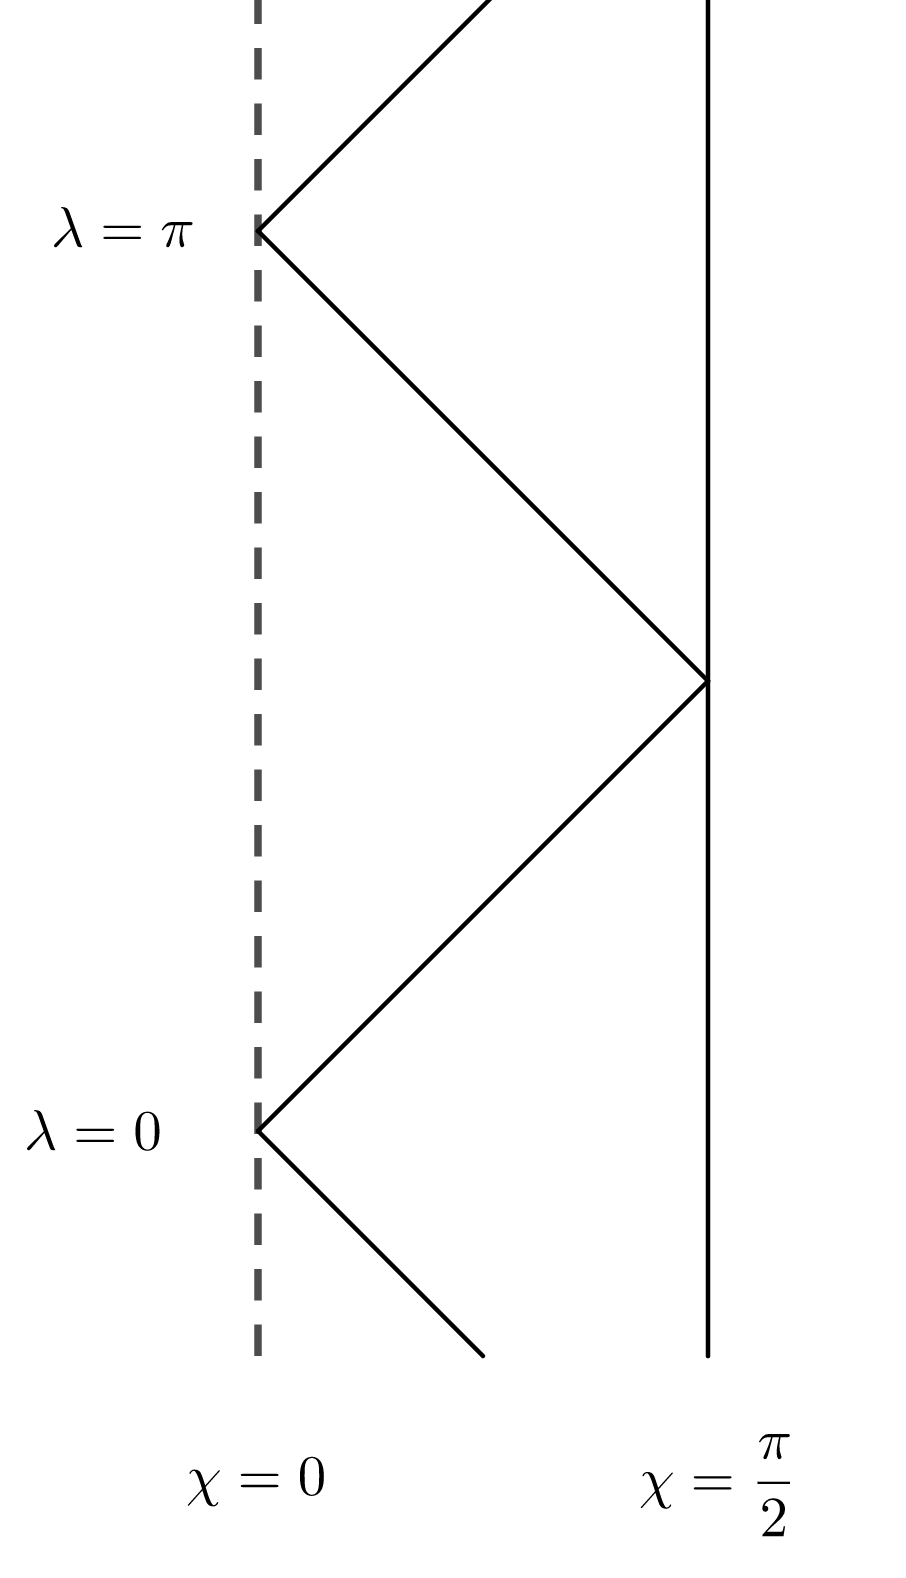
\includegraphics[width=0.35\textwidth]{../pics/AdS3_Pen.png}
%
\caption{Conformal diagram of anti-de Sitter space. We see that light rays can emerge at conformal infinity $\mathcal{J}$ at any $\lambda$, and subsequently terminate at $\mathcal{J}$ at a later $\lambda$. Thus, there are no \textbf{Cauchy surfaces} in $AdS_3$, and consequently we do not have well-posed initial value problems on the $AdS_3$ spacetime.}
%
\label{fig:penrose_ads}
%
\end{figure}
%
%
\noindent
%
Looking at the above conformal digram, we see a very interesting causal property of $AdS_3$, namely that conformal infinity $\mathcal{J}$ is a time-like hypersurface. As a consequence of this fact, $AdS_3$ is not globally hyperbolic, meaning that it has no \textbf{Cauchy surfaces}. This is because there exists null geodesics which both emerge and terminate at $\mathcal{J}$. Thus, we do not have well-posed initial value problems on the $AdS_3$ in terms of information specified on a Cauchy surface. Later in section 4.1, when we compute \textbf{Green's functions} on the BTZ spacetime, the fact that $AdS_3$ is not globally hyperbolic will force us to choose boundary condition for the scalar field at infinity. More details will follow in said section.

%%%%%%%%%%%%%%%%%%%%%%%%%%%%%%%%%%%%%%%%%%%%%%%%%%%%%%%%%%%%%%%%%%%%%%%%%%%%%%%%%%%%%%%%%%
%\subsubsection{Describtion in terms of SL(2, R)}
%Points in the ambient space can be represented by $2 \times 2$ real matrices. Let us for future convinience introduce the following basis on the space of $2 \times 2$ real matrices:
%%
%%
%\begin{equation}
%\gamma^0 = \frac{1}{l} \, \bigg( \begin{array}{cc}
%1 & 0 \\
%0 & 1
%\end{array} \bigg)
%\; , \;
%\gamma^1 = \frac{1}{l} \, \bigg( \begin{array}{cc}
%0 & 1 \\
%-1 & 0
%\end{array} \bigg)
%\; , \;
%\gamma^2 = \frac{1}{l} \, \bigg( \begin{array}{cc}
%1 & 0 \\
%0 & -1
%\end{array} \bigg)
%\; , \;
%\gamma^3 = \frac{1}{l} \, \bigg( \begin{array}{cc}
%0 & 1 \\
%1 & 0
%\end{array} \bigg)
%\end{equation}
%%
%%
%Where $l \in \mathbb{R}_+$. We can now represent a points in the ambient space by a matrix $\mathbf{X}$:
%%
%%
%\begin{equation}
%\mathbf{X} = x_a \, \gamma^a
%= \frac{1}{l} \, \bigg( \begin{array}{cc}
%x_0 + x_2 & x_1 + x_3 \\
%-x_1 + x_3 & x_0 - x_2
%\end{array} \bigg)
%\quad , \quad
%||x||^2
%= \eta^{ab}_{2,2} \, x_a \, x_b
%= -l^2 \, \det(\mathbf{X})
%\end{equation}
%%
%%
%Where $a \in \{ 0,1,2,3 \}$. From the above relations, we see that the norm preserving transformations on the abient space (\textit{elements of $SO(2,2)$}) can be reresented by elements of $\mathrm{SL}(2, \mathbb{R}) \times \mathrm{SL}(2, \mathbb{R}) / \mathbb{Z}_2$, acting on the $2 \times 2$ matrices in the following way:
%%
%%
%\begin{equation}
%\mathbf{X} \to  \rho_R \, \mathbf{X} \rho_L
%\quad , \quad
%(\rho_R, \rho_L) \in \mathrm{SL}(2, \mathbb{R}) \times \mathrm{SL}(2, \mathbb{R}) / \mathbb{Z}_2
%\end{equation}
%%
%%
%From the definition above, it is clear that the $\mathbb{Z}_2$ identification must be $(\rho_L, \rho_R) \sim (-\rho_L, -\rho_R)$. The constraint (\ref{anti-de sitter}) can now be expressed in terms of the $2 \times 2$ real matrices defined above:
%%
%%
%\begin{equation}
%\eta^{ab}_{2,2} \, x_a \, x_b
%= -l^2
%\quad \Rightarrow \quad
%\det(\mathbf{X}) = 1
%\end{equation}
%%
%%
%It is evident that the entire isometry group (\textit{apart from the reflections}) of $adS$ is the $SO(2,2)$ group.
%%%%%%%%%%%%%%%%%%%%%%%%%%%%%%%%%%%%%%%%%%%%%%%%%%%%%%%%%%%%%%%%%%%%%%%%%%%%%%%%%%%%%%%%%%%

\subsubsection{Constructing the BTZ spacetime}
As we have already mentioned previously, any solution to the vacuum Einstein Equatins in (2+1) must be locally isomorphic to $AdS_3$. Thus, the BTZ spacetime must also be locally isomorphic to $AdS_3$. However, there is no guarantee that the global structure of the BTZ spacetime should be related to that of $AdS_3$ in any simple way. Fortunately, it turns out that the global structures of BTZ and $AdS_3$ actually \textit{is} related in a simple way. This is most easilly seen by covering the hypersurface (\ref{anti-de sitter}) with a set of coordinates $(t, r, \phi)$, as defined in appendix B. It is easy to verify that the pull-back of the metric (\ref{ambient_metric}) onto the $AdS_3$ hypersurface, using the coordinates $(t, r, \phi)$, recovers the BTZ metric (\ref{btz_metric}) in each of the regions \textbf{I}, \textbf{II} and \textbf{III}, with $\Lambda = -\ell^{-2}$. In order for the $(t, r, \phi)$ coordinates to cover all of $AdS_3$, they must have the following ranges:
%
%
\begin{equation}
r \in (0, r_-) \cup (r_-, r_+) \cup (r_+, \infty)
\quad , \quad
\phi \in (-\infty, \infty)
\quad , \quad
t \in (-\infty, \infty)
\end{equation}
%
%
This is exactly the ranges of the  Schwarzschild-like coordinates on the BTZ spacetime, except that $\phi$ is here an uncompact coordinate. Thus, we arrive at the amazing fact that the BTZ spacetime can be constructed from $AdS$, by identifying points such that $\phi \sim \phi + 2 \pi$. This fact will greatly aid us in section 4.1, when we set out to find Green's functions on the BTZ spacetime.


% section 3: Properties
\newgeometry{top=2cm,left=2cm,right=2cm,bottom=2cm} 
%
\section{Classical properties of the BTZ spacetime}
As mentioned back in section 2.2, the BTZ spacetime has many features in common with black hole solutions in (3+1) dimensions, and in particular the Kerr black hole. As was pointed out during the derivation of the BTZ metric in section 2.2, a mass $M$ and angular momentum $J$ can be defined for the spacetime. It also posses two event horizons at:
%
%
\begin{equation}
r^2_{\pm}
=  \frac{\ell^2}{2} \, \left[
M \pm \sqrt{M^2 - \left(\frac{J}{\ell} \right)^2}
\right]
\end{equation}
As was also shown in section 2.2. Just like the Kerr black hole, the BTZ black hole also posses an \textbf{ergosphere}, which is a region between the outer horizon and the so-called \textbf{ergo shell}. In Schwarzschild-like coordinates, the ergo shell is defined as the hypersurafce on which $\partial_t$ becomes null, and thus:
%
%
\begin{equation}
g_{tt}(r) = 0
\quad \Rightarrow \quad
-M + \frac{r^2}{\ell^2} = 0
\quad \Rightarrow \quad
r_{erg}^2 = M \, \ell^2 \geq r_+^2
\end{equation}
%
%
The interesting thing about the ergosphere is that time-like curves in this region must partially be moving in the direction of $\partial_{\phi}$, as the only negative metric component in this region is $g_{t\phi}$.\newline
We have now exhausted the list of interesting properties of the BTZ spacetime which can easilly be extracted from its mettric. To better be able to investigate the causal properties of the BTZ spacetime, we now proceed to derive its conformal digram.

%%%%%%%%%%%%%%%%%%%%%%%%%%%%%%%%%%%%%
%\subsection{Mass and angular momentum}
%In order to properly define the mass and spin of the BTZ spactime, we will have to employ the \textbf{Chern-Simons formulation} of (2+1) dimensional gravity. As already discussed in section 2.3, the isometry group of $\widetilde{adS}$ is $SO(2,2)$. We first note that the Lie algebra $so(2,2)$ is isomorphic to the Lie algebra $iso(2,1)$; the Lie algebra of the (2+1) dimensional \textbf{Pioncaré group}. We can now use this fact to construct a $SO(2,2)$ 1-form potential usning the connection 1-forms ${\omega^i}_j$ and the triad frame $\epsilon^i$:
%%
%%
%\begin{equation}
%A := \frac{1}{2} \, \omega^{ij} \, \mathcal{J}_{ij} + \frac{1}{l} \, e^i \, \mathcal{P}_i
%\end{equation}
%%
%%
%Where $\mathcal{J}_{ij}$ and $\mathcal{P}_i$ are the rotation and translation generators of $iso(2,1)$ respectivly. It can now be shown that the \textbf{Einstein-Hilbert action} can be rewritten (\textit{up to boundary terms}) using a 3-form lagrangian $L(A)$ constructed from the potential $A$:
%%
%%
%\begin{equation}
%I_{EH}[A] = \frac{l}{2 \pi} \, \int_{\mathcal{M}} L(A)
%= \frac{l}{2 \pi} \, \int_{\mathcal{M}} \mathrm{Tr} \bigg[ A \wedge \mathrm{d}A + \frac{2}{3} \, A \wedge A \wedge A \bigg]
%\end{equation}
%%
%%
%Where $\mathrm{Tr}$ is defined such that $\mathrm{Tr}(\mathcal{J}_{ij} \, \mathcal{P}_k) = \varepsilon_{ijk}$, $\mathrm{Tr}(\mathcal{J}_{ij} \, \mathcal{J}_{kl}) = 0$ and $\mathrm{Tr}(\mathcal{P}_i \, \mathcal{P}_j) = 0$. It can now be shown that the variation of the lagrangian $L$ under the flow of a Killing vector $X$ is given by:
%%
%%
%\begin{equation}
%\mathcal{L}_X \, L = \mathrm{d}(i_X \, L) + i_x \, \mathrm{d}L = \mathrm{d}J = 0
%\quad , \quad
%J = i_X \, L = \frac{l}{2 \pi} \, \mathrm{d}\mathrm{Tr}(A \, i_X \, A)
%\end{equation}
%%
%%
%Where $i_X$ is the interior product (\textit{contraction operator}). We can now use the conserved current $J$ to define a conserved quantity corresponding to any given Killing vector $X$, by integrating over a spatial hyper-surface $\Sigma$:
%%
%%
%\begin{equation}
%Q[X] := \int_{\Sigma} J
%= \frac{l}{2 \pi} \, \int_{\partial \Sigma} \mathrm{d}\mathrm{Tr}(A \, i_X \, A)
%= \frac{1}{2 \pi} \, \int_{\partial \Sigma} \frac{1}{2} \varepsilon_{ijk} \, \big(
%\omega^{ij} \, \epsilon^k(X)
%+ \omega^{ij}(X) \, \epsilon^k
%\big)
%\end{equation}
%%
%%
%We can now define the mass and angular momentum of the BTZ spacetime using its two Killing vectors $\partial_t$ and $\partial_{\phi}$. In section 2.2, we defined a triad for the BTZ metric and found the corresponding connection 1-forms, and using those expressions we find that:
%%
%%
%\begin{equation}
%\frac{1}{2} \varepsilon_{ijk} \, \big(
%\omega^{ij} \, \epsilon^k(\partial_t)
%+ \omega^{ij}(\partial_t) \, \epsilon^k
%\big)
%= M \, \mathrm{d}\phi + \frac{J}{l^2} \, \mathrm{d}t
%\end{equation}
%%
%%
%\begin{equation}
%\frac{1}{2} \varepsilon_{ijk} \, \big(
%\omega^{ij} \, \epsilon^k(\partial_{\phi})
%+ \omega^{ij}(\partial_{\phi}) \, \epsilon^k
%\big)
%= J \, \mathrm{d}\phi + M \, \mathrm{d}t
%\end{equation}
%%
%%
%Thus, if we choose $\Sigma$ to be a surface of constant $t$, we can integrate the above expressions to find:
%%
%%
%\begin{equation}
%Q[\partial_t] = M
%\quad , \quad
%Q[\partial_{\phi}] = J
%\end{equation}
%%%%%%%%%%%%%%%%%%%%%%%%%%%%%%%%%%%%%

\subsection{Causal structure of the spacetime}
We will here focus on deriving a conformal digram for the case of $J=0$; the static BTZ black hole. The metric for the static BTZ black hole is given by:
%
%
\begin{equation}\label{static_btz}
ds^2 = -f^2(r) \, \mathrm{d}t^2
+ f^{-2}(r) \, \mathrm{d}r^2
+ r^2 \mathrm{d}\phi^2
\quad , \quad
f^2(r) = -M + \frac{r^2}{\ell^2}
\end{equation}
%
\begin{equation*}
-\infty < t < \infty \, , \quad 0 < r < \infty \, , \quad 0 \leq \phi < 2 \pi
\end{equation*}
%
%
Because this metric is so similar to the (3+1)-dimensional Schwarzschild black hole, we can follow the usual derivation as seen in \cite{GR} of Kruskal coordinates and a Penrose diagram quite closely.\newline
%
%
%
Before we start, we note that just like in the Schwarzschild metric, there appears to be a singularity at $r = r_+ = \ell \, \sqrt{M}$. As was the case with Schwarzschild, this is merely a coordinate singularity. Because it is shown in the exact same way as for Schwarzschild, we will not go through any trouble showing it explicitly, but it will be apparent once we see the conformal diagram.
We start by introducing a so-called turtoise coordinate $r^*$, such that:
%
%
\begin{equation}
f^2(r) \, (\mathrm{d}r^*)^2
= f^{-2}(r) \, \mathrm{d}r^2
\quad \Rightarrow \quad
\frac{\mathrm{d}r^*}{\mathrm{d}r} = f^{-2}(r)
\end{equation}
%
%
\begin{equation}
\Rightarrow \quad
r^*(r) = \int \frac{1}{\frac{r^2}{\ell^2} - M} dr =
\frac{\ell^2}{2 r_+} \int \frac{1}{r - r_+} - \frac{1}{r + r_+} dr =
\frac{\ell^2}{2 r_+} \ln \left( \frac{|r - r_+|}{r + r_+} \right)
\end{equation}
%
%
We see that the $r^*(r)$ is singular at $r = r_+$, so we only look at the case $r > r_+$, for which we do not need the absolute value.
%
%
%
By changing to the turtoise coordinate, we can bring the metric to the form:
%
%
\begin{equation}
ds^2 = f^2(r) \, \left[- \mathrm{d}t^2 + (\mathrm{d}r^*)^2 \right] + r^2(r^*) \, \mathrm{d}\phi^2
\end{equation}
\begin{equation*}
-\infty < t < \infty
\quad , \quad
-\infty < r^* < 0
\end{equation*}
%
%
%
It it is now straightforward to define a pair of null coordinates $v$ and $u$, using the above metric:
%
%
\begin{equation}
v = t + r^*
\qquad,\qquad
u = t - r^*
\end{equation}
%
%
In terms of the new null coordinates $v$ and $u$, the static BTZ metric now takes the following form:
%
%
\begin{equation}
ds^2 = - \frac{f^2(r)}{2} \, \left[ \mathrm{d}u \, \mathrm{d}v
+ \mathrm{d}v \, \mathrm{d}u \right]
+ r^2 \, \mathrm{d}\phi^2
\end{equation}
%
\begin{equation*}
-\infty < u, v < \infty 
\quad , \quad
v < u
\end{equation*}
%
%
We note that $r$ is now to be interpreted as an implicit function of $v$ and $u$, with the following relation:
%
%
\begin{equation}
\frac{1}{2}(v - u)
= \frac{\ell^2}{2 r_+} \ln \left( \frac{r - r_+}{r + r_+} \right)
\end{equation}
%
%
%
Just like in the Schwarzschild case, the apparent coordinate singularity at $r = r_+$ is moved to infinity in these coordinates. Fixing it requires us to write $u$ and $v$ in terms of our initial coordinates $t$ and $r$:
%
%
\begin{equation}
v = t + r^*
= t + \frac{\ell^2}{2 r_+} \ln \left( \frac{r - r_+}{r + r_+} \right)
\qquad , \qquad 
u = t - r^*
= t - \frac{\ell^2}{2 r_+} \ln \left( \frac{r - r_+}{r + r_+} \right)
\end{equation}
%
%
%
We see now that a clever choice of coordinates $v'$ and $u'$, might be given by the following:
%
%
\begin{equation}
v' = \exp \left( \frac{r_+ v}{\ell^2}\right) \qquad , \qquad
u' = - \exp \left( \frac{-r_+ u}{\ell^2}\right)
\end{equation}
%
%
These can be expressed in terms of the original coordinates $t$ and $r$, in the following way:
%
%
\begin{equation}
v' = \sqrt{\frac{r - r_+}{r + r_+}} \exp \left( \frac{r_+ t}{\ell^2}\right) \qquad , \qquad
u' = -\sqrt{\frac{r - r_+}{r + r_+}} \exp \left( \frac{- r_+ t}{\ell^2}\right)
\end{equation}
%
%
In terms of the coordinates $v'$ and $u'$, the static BTZ metric now takes the following form:
%
%
\begin{equation}
ds^2 = - \frac{f^2(r)}{2} \, \frac{\ell^4}{r_+^2} \,
\left( \frac{r + r_+}{r - r_+} \right) \left[ \mathrm{d}u' \mathrm{d}v' + \mathrm{d}v' \mathrm{d}u'\right]
+ r^2 \, \mathrm{d}\phi^2
\end{equation}
%
\begin{equation*}
0 < v' < \infty
\quad , \quad
-\infty < u' < 0
\quad , \quad
v' \, u' < -1
\end{equation*}
%
%
%
We can simplify the above metric a bit by realizing that:
%
%
\begin{equation}\label{fsimply}
f^2(r) = -M + \frac{r^2}{\ell^2}
= \frac{r^2 - r_+^2}{l^2}
= \frac{(r - r_+)(r + r_+)}{\ell^2}
= \frac{(r + r_+)^2}{\ell^2} \left( \frac{r - r_+}{r + r_+} \right)
\end{equation}
%
%
Using the above expression for $f^2(r)$, we now find that:
%
%
\begin{equation} \label{premetric}
ds^2 = - \frac{\ell^2}{2} \, \frac{(r + r_+)^2}{r_+^2} \, \left[ \mathrm{d}u' \mathrm{d}v' + \mathrm{d}v' \mathrm{d}u' \right]
+ r^2 \mathrm{d}\phi^2
\end{equation}
%
%\begin{equation*}
%0 < v' < \infty
%\quad , \quad
%-\infty < u' < 0
%\quad , \quad
%0 \leq \phi < 2 \pi
%\end{equation*}
%
%
%
It is now apparent that $r = r_+$ is not a real singularity, since the metric is not singular for this value of $r$ in these coordinates. To get the Kruskal.like coordinates for the BTZ black holes, we just need to change back into a set of one time-like and two space-like coordinates, using the combination:
%
%
\begin{equation}\label{RandT}
T = \frac{1}{2} \, (v' + u') \qquad , \qquad
R = \frac{1}{2} \, (v' - u')
\end{equation}
%
%
We can now write the coordinates $T$ and $R$, in terms of the original coordinates $t$ and $r$:
%
%
\begin{equation}\label{RightT}
T = \frac{1}{2} \, \sqrt{\frac{r - r_+}{r + r_+}} \, \left[
\exp \left( \frac{r_+ t}{\ell^2}\right)
-
\exp \left( \frac{- r_+ t}{\ell^2}\right)
\right] 
= \sqrt{\frac{r - r_+}{r + r_+}} \, \sinh \left( \frac{r_+ t}{\ell^2}\right)
\end{equation}
%
%
\begin{equation}\label{RightR}
R = \frac{1}{2} \, \sqrt{\frac{r - r_+}{r + r_+}} \, \left[
\exp \left( \frac{r_+ t}{\ell^2}\right)
+
\exp \left( \frac{- r_+ t}{\ell^2}\right)
\right] 
= \sqrt{\frac{r - r_+}{r + r_+}} \, \cosh \left( \frac{r_+ t}{\ell^2}\right)
\end{equation}
%
%
The metric for the static BTZ balck hole, now takes a particularly simple form, in terms of $T$ and $R$:
%
%
\begin{equation}
ds^2 = \ell^2 \, \frac{(r + r_+)^2}{r_+^2} \, \left[
-\mathrm{d}T^2
+ \mathrm{d}R^2 \right]
+ r^2 \, \mathrm{d}\phi^2
\end{equation}
%
\begin{equation*}
-\infty < T, R < \infty
\quad , \quad
-1 < R^2 - T^2 < 1
\quad , \quad
0 \leq \phi < 2 \pi
\end{equation*}
%
%
%
It is easily seen from (\ref{RightR}) and (\ref{RandT}), that $R^2 - T^2 > 0$ and $R > 0$, for $r > r_+$. But space-like geodesics can reach $R = 0$ at finite parameter value, so there must be more spacetime beyond this. We can cover this other patch by a set of coordinates similar to (\ref{RightR}) and (\ref{RightT}), but with a minus sign on each coordinate (\textit{so that $R < 0$; we see that these two patches do not overlap}). \newline
When we defined the turtoise coordinate $r^*$, we noted that it was singular at $r = r_+$, and chose to look at only $r > r_+$. Had we instead chosen $0 < r < r_+$, we would have simply swapped the order of $r_+$ and $r$ when we removed the absolute value, such that:
%
%
\begin{equation}
r^* = \frac{\ell^2}{2 r_+} \ln \left( \frac{r_+ - r}{r + r_+} \right)
\end{equation}
%
%
This would have given us a minus sign in (\ref{fsimply}), which would have lead to us swapping the definitions of $T$ and $R$ in (\ref{RandT}), and consequently the definitions of $T$ and $R$ in terms of $t$ and $r$ would be swapped as well. This would correspond to a patch in which $R^2 - T^2 < 0$ and $T > 0$. In this patch of spacetime, it is possible for time-like geodesics to reach $T = 0$ at finite parameter value, so there must be more spacetime beyond this as well. We can, once again, cover this new patch by simply adding a minus sign to each coordinate $T$ and $R$. This leaves us with the maximally extended spacetime for the static BTZ black hole, consisting of four patches with the following coordinates:\newline
\newline
%
%
\noindent
\textbf{I} \qquad ($r_+ < r$)
%
\begin{equation}
T = \sqrt{\frac{r - r_+}{r + r_+}} \sinh \left( \frac{r_+ t}{\ell^2}\right)
\qquad , \qquad
R = \sqrt{\frac{r - r_+}{r + r_+}} \cosh \left( \frac{r_+ t}{\ell^2}\right)
\end{equation}
%
%
\textbf{II} \qquad ($0 < r < r_+$)
%
\begin{equation}
T = \sqrt{\frac{r_+ - r}{r + r_+}} \cosh \left( \frac{r_+ t}{\ell^2}\right)
\qquad , \qquad
R = \sqrt{\frac{r_+ - r}{r + r_+}} \sinh \left( \frac{r_+ t}{\ell^2}\right)
\end{equation}
%
%
\textbf{III} \qquad ($r_+ < r$)
%
\begin{equation}
T = - \sqrt{\frac{r - r_+}{r + r_+}} \sinh \left( \frac{r_+ t}{\ell^2}\right)
\qquad , \qquad
R = - \sqrt{\frac{r - r_+}{r + r_+}} \cosh \left( \frac{r_+ t}{\ell^2}\right)
\end{equation}
%
%
\textbf{IV} \qquad ($0 < r < r_+$)
%
\begin{equation}
T = - \sqrt{\frac{r_+ - r}{r + r_+}} \cosh \left( \frac{r_+ t}{\ell^2}\right)
\qquad , \qquad
R = - \sqrt{\frac{r_+ - r}{r + r_+}} \sinh \left( \frac{r_+ t}{\ell^2}\right)
\end{equation}\newline
%
%
\begin{figure}[h!]
%
\centering
%
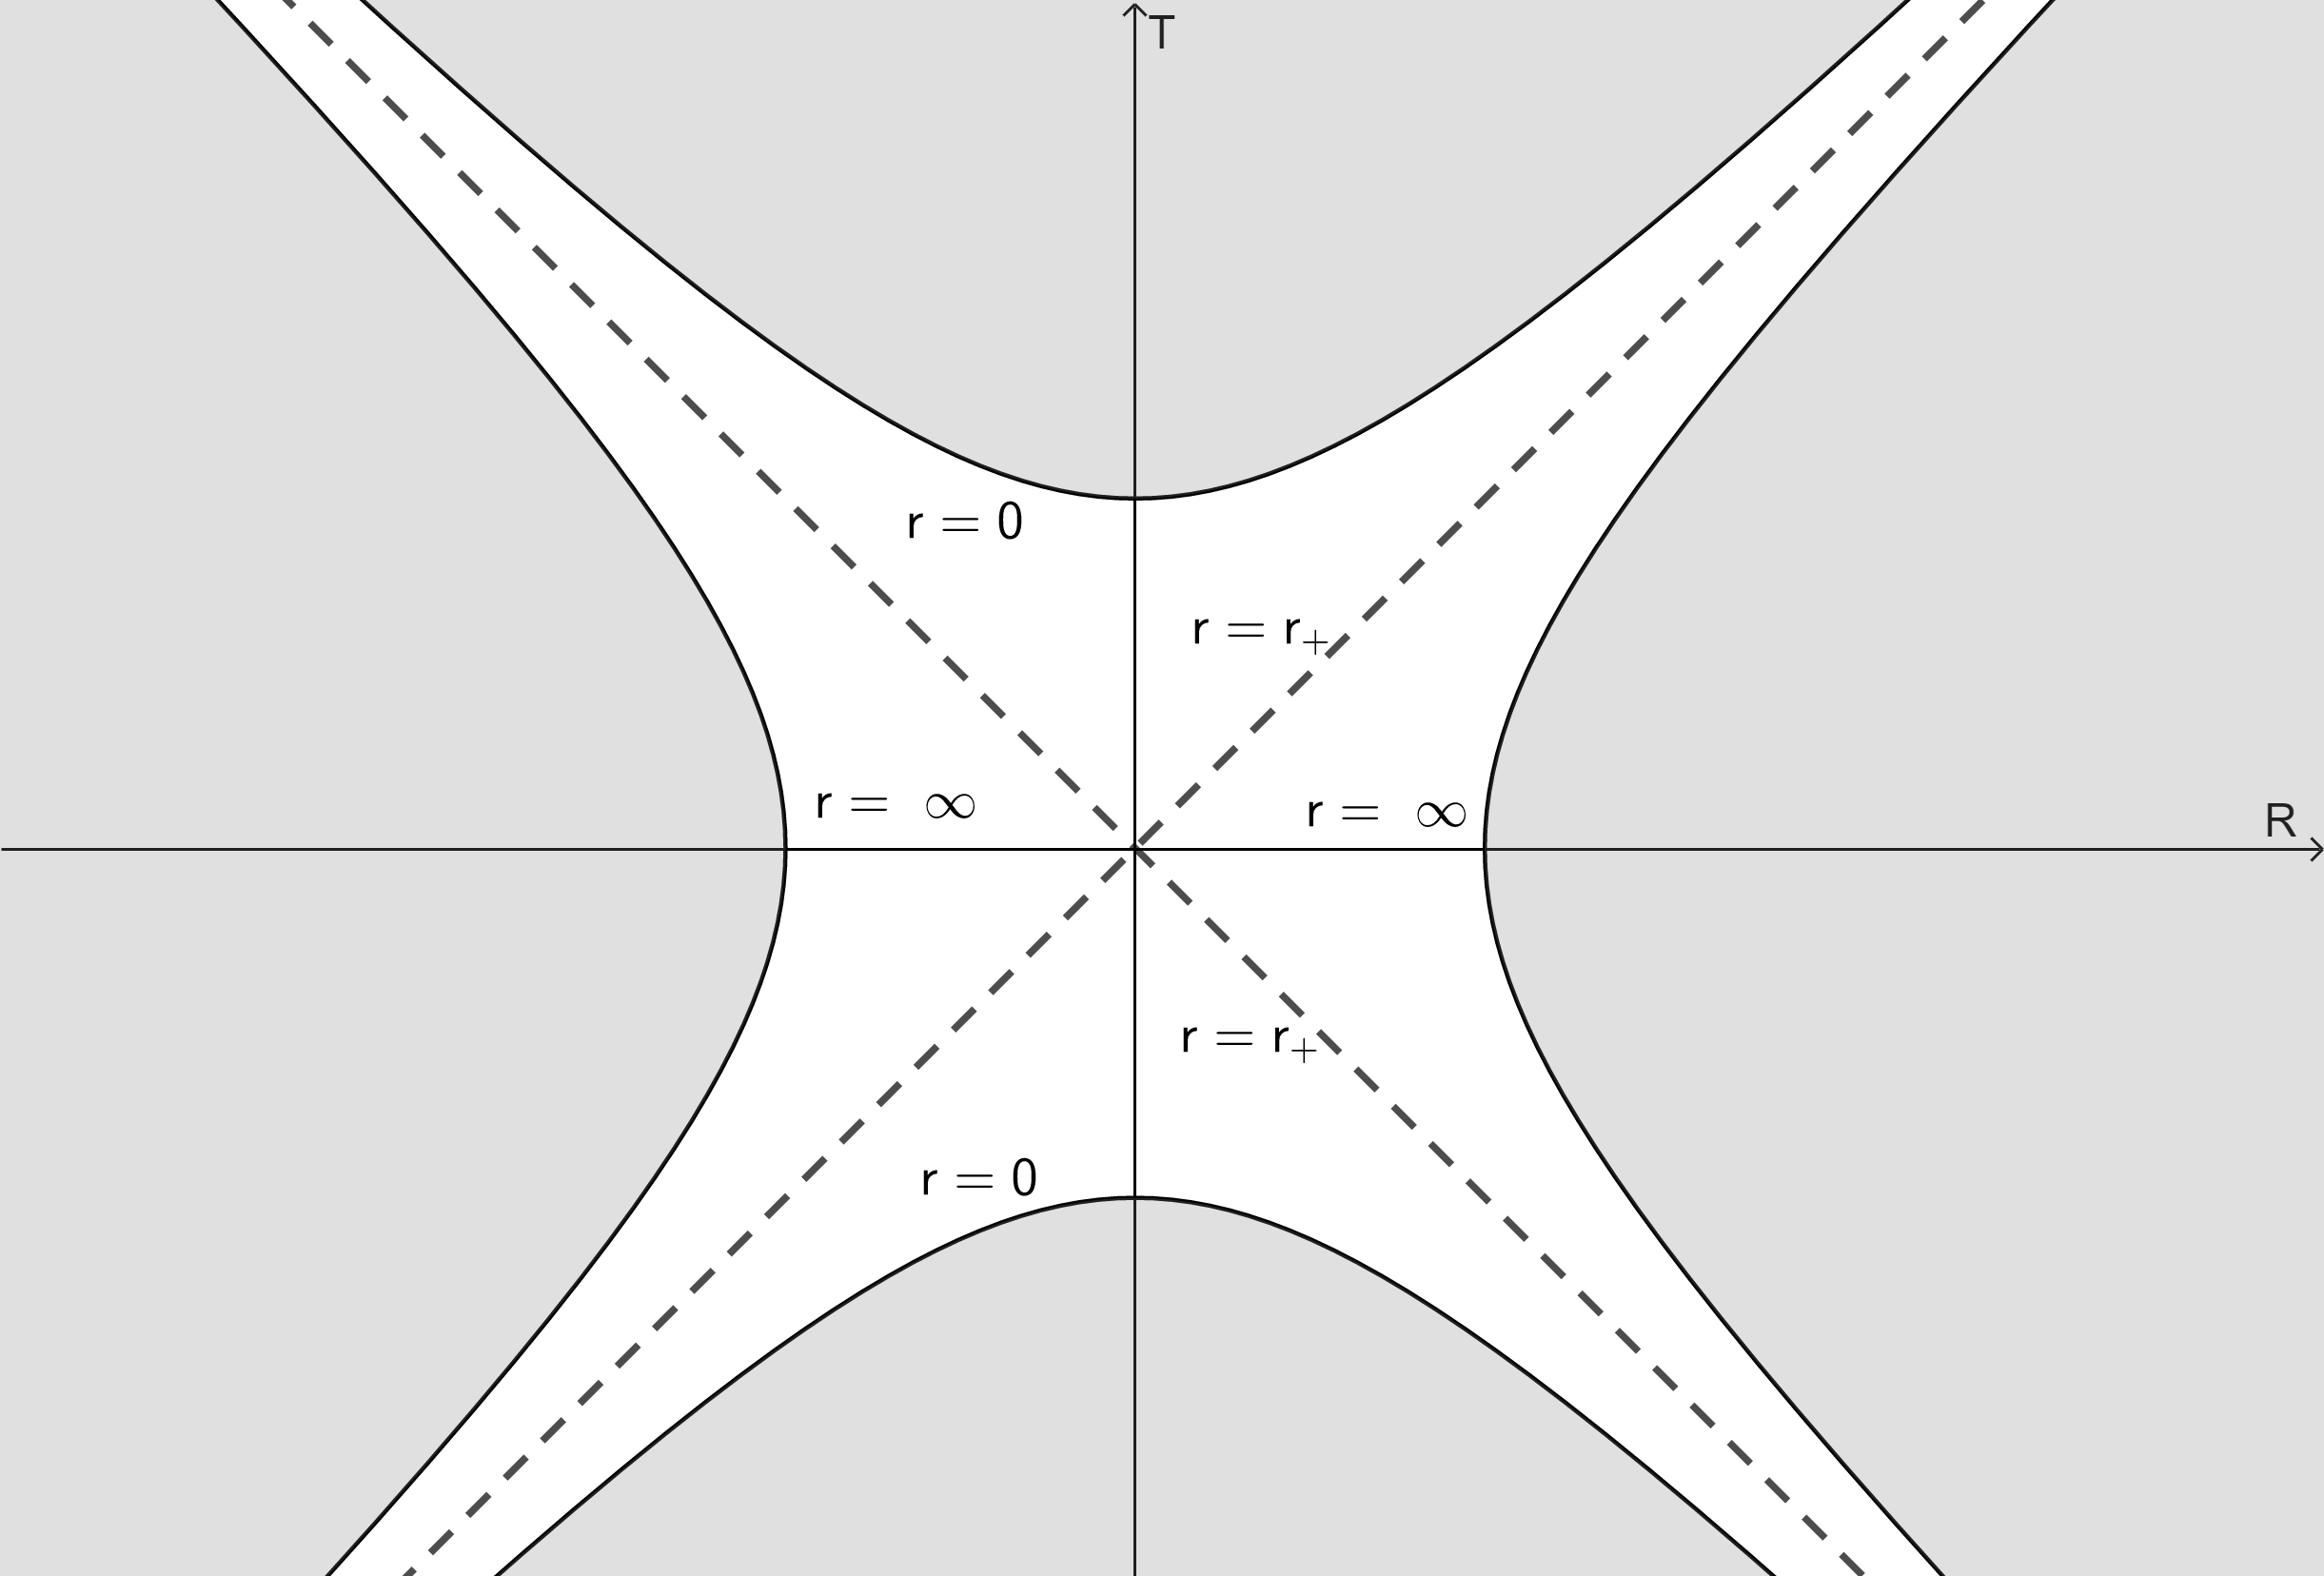
\includegraphics[width=0.80\textwidth]{../pics/Kruskal_static.png}
%
\caption{The Kruskal-diagram for the static BTZ black hole. Light rays move on $45^{\circ}$ lines in these coordinates. The past and future event horizons are null surfaces located at $r=r_+$. The grey areas are not part of the spacetime.}
%
\label{fig:kruskal_static}
%
\end{figure}\newline \noindent
%
%
Patch I and III corresponds to two different asymptotically $AdS_3$ parts of the spacetime (\textit{as will be clear when the conformal digram is constructed}), while II and IV are the black and white hole respectively. In patch I and III, we see that $r = const$ corresponds to $0 < R^2 - T^2 = const < 1$, while $t = const$ corresponds to $-1 < T / R = const < 1$. This means that constant $r$ curves are hyperbolas while constant $t$ curves are lines intersecting the origin, just as in the Schwarzschild case. The point at $r = 0$ lies in patch II and IV, and are described by the hyperbolas:
%
%
%\begin{equation}
%T_0 = \cosh \left( \frac{r_+ t}{\ell^2} \right) \qquad , \qquad
%R_0 = \sinh \left( \frac{r_+ t}{\ell^2} \right)
%\end{equation}
\begin{equation}
R^2 - T^2 = -1
\end{equation}
%
%
%
Which is again just like the Schwarzschild case. Different from the Schwarzschild case however, is $r = \infty$, which usually lies at $R^2 - T^2 = \infty$, but now lies in patch I and III, and are described by:
%
%
%\begin{equation}
%T_\infty = \sinh \left( \frac{r_+ t}{\ell^2} \right) \qquad , \qquad
%R_\infty = \cosh \left( \frac{r_+ t}{\ell^2} \right)
%\end{equation}
\begin{equation}
R^2 - T^2 = 1
\end{equation}
%
%
%
If we want to construct a conformal diagram for the static BTZ spacetime, we can follow the approach of not only Schwarschild but also flat space, and make another coordinate transformation:
%
%
\begin{equation}
v' = \tan \left( r_+ V \right)
\qquad , \qquad
u' = \tan \left( r_+ U \right)
\end{equation}
%
%
\begin{equation}
\Rightarrow \quad
\mathrm{d} v' = \frac{r_+}{\cos^2(r_+ V)} \mathrm{d}V
\qquad , \qquad
\mathrm{d} u' = \frac{r_+}{\cos^2(r_+ U)} \mathrm{d}U
\end{equation}
%
%
\begin{equation}
\Rightarrow \quad
\mathrm{d} v' \mathrm{d} u' + \mathrm{d} u' \mathrm{d} v' =
\frac{{r_+}^2}{\cos^2(\frac{V}{r_+}) \cos^2(\frac{U}{r_+})} \left[ \mathrm{d}V \mathrm{d}U + \mathrm{d}U \mathrm{d}V \right]
\end{equation}
%
%
We can now write the metric (\ref{premetric}), using the coordinates $V$ and $U$, in the follow way:
%
%
\begin{equation}
ds^2 = - \frac{\ell^2}{2} \, \frac{(r + r_+)^2}{\cos^2(r_+ V) \cos^2(r_+ U)} \left[ \mathrm{d}V \mathrm{d}U + \mathrm{d}U \mathrm{d}V \right]
+ r^2  \, \mathrm{d}\phi^2
\end{equation}
%
\begin{equation*}
0 < V < \pi/2
\quad , \quad
-\pi/2 < U < 0
\quad , \quad
0 \leq \phi < 2 \pi
\end{equation*}
%
%
We now make one last transformation to one time-like and one space-like coordinate, $T'$ and $R'$:
%
%
\begin{equation}
V = \frac{1}{2} \, (T' + R')
\qquad , \qquad
U = \frac{1}{2} \, (T' - R')
\end{equation}
%
%
In terms of the time-like coordinate $T'$ and space-like coordinate $R'$, the metric finally takes the form:
%
% This equation should not have two numbers (fixed)
%
\begin{align}
ds^2 & = \omega^{-2} \, \left[- (\mathrm{d}T')^2 + (\mathrm{d}R')^2 \right]
+ r^2 \, \mathrm{d}\phi^2
\notag\\
\omega^{-2} & = \frac{2 \, \ell^2 \, (r + r_+)^2}{\left[ \cos(r_+ T') + \cos(r_+ R') \right]^2}
\end{align}
%
\begin{equation*}
-\pi/2 < T', R' < \pi/2
\quad , \quad
0 \leq \phi < 2 \pi
\end{equation*}
%
%
If we omit the angular part of the above metric, we now easily see that the rest of the metric is related by the conformal factor $\omega^2$ to the metric of flat two dimensional Minkowski space:
%
%
\begin{equation}
\tilde{ds}^2 = - (\mathrm{d}T')^2 + (\mathrm{d}R')^2
\end{equation}
\begin{equation*}
-\pi/2 < T', R' < \pi/2
\end{equation*}
%
%
Having found these coordinates, we can now draw the conformal diagram for the static BTZ Black Hole. It will look like the Schwarzschild Black Hole near the event horizon, but will have the same structure at conformal infinity as $AdS_3$:
%
%
\begin{figure}[h!]
%
\centering
%
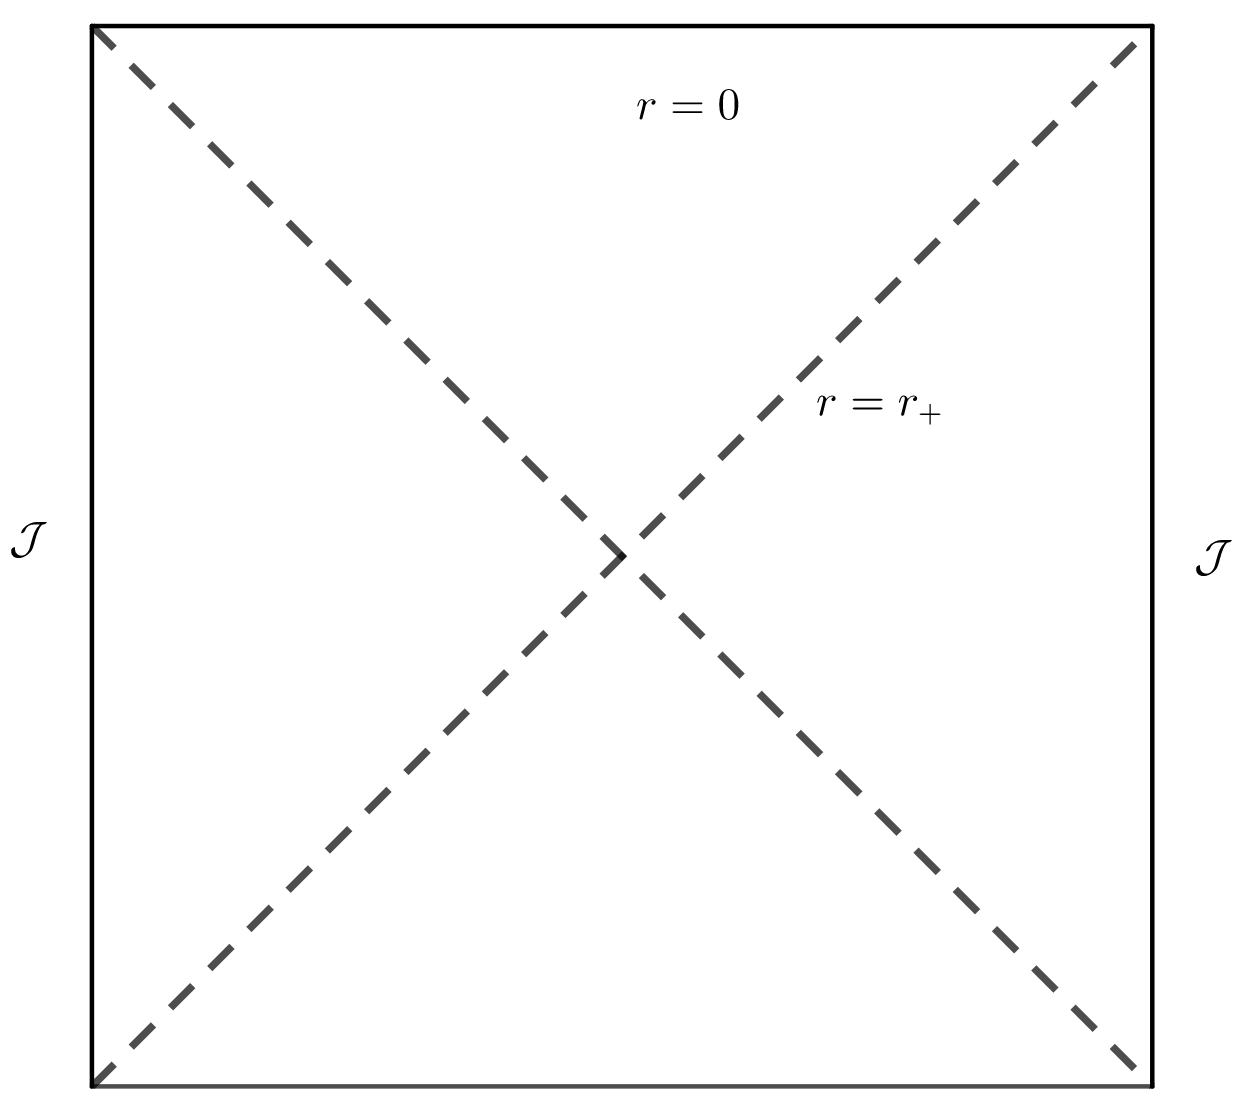
\includegraphics[width=0.6\textwidth]{../pics/BTZ_stat_Pen.png}
%
\caption{The conformal diagram for the static BTZ black hole. The past and future event horizons are again located at $r=r_+$. In this digram, we now see that the spacetime is asymptotically $AdS_3$.}
%
\label{fig:pen_btz_static}
%
\end{figure}
%
%
%%%%%%%%%%%%%%%%%%%%%%%%%%%%%%%%%%%%%
%\begin{figure}[h!]
%%
%\centering
%%
%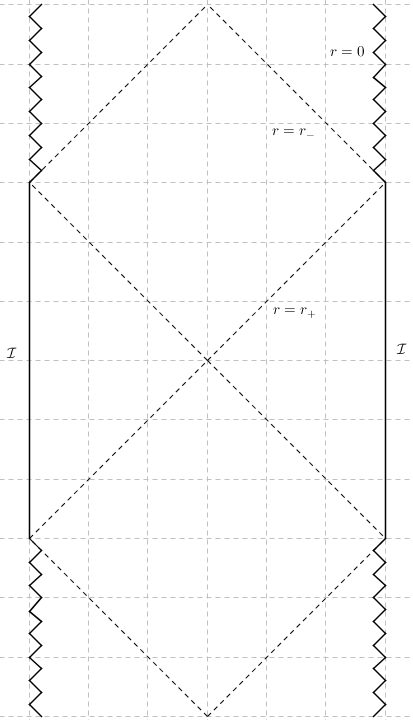
\includegraphics[width=0.6\textwidth]{../pics/BTZ.png}
%%
%\caption{The conformal diagram for the rotating BTZ black hole. In this digram, we can now easily see that the spacetime is asymptotically $AdS_3$.}
%%
%\label{fig:pen_btz}
%%
%\end{figure}
%%%%%%%%%%%%%%%%%%%%%%%%%%%%%%%%%%%%%

\newpage

\subsection{Singularities}
As we have already seen in the previous subsection, the apparent singularities at the inner and outer horizon are coordinate dependent singularities, as is also the case for black hole solutions in (3+1) dimensions. Therefore, one would expect the curvature to stay finite on the horizons. In order to check this, and to identify any other potential curvature singularites of the BTZ black hole, we can compute the \textbf{curvature invariant} $R_{ijkl} \, R^{ijkl}$. Using the expression we obtained in section 1.3, for the Riemann tensor associated with vacuum solutions to Einsteins Equations, we find that:
%
%
\begin{equation}
R_{ijkl} \, R^{ijkl}
= \Lambda^2 \, (g_{\rho\mu} \, g_{\nu\sigma} - g_{\rho\nu} \, g_{\mu\sigma}) \, 
(g^{\rho\mu} \, g^{\nu\sigma} - g^{\rho\nu} \, g^{\mu\sigma})
= 12 \, \Lambda^2
\end{equation}
%
%
It is now evident, that the BTZ black hole has no curvature singularities anywhere. This is very different from black holes in (3+1) dimensions, which all possess some kind of curvature singularity in their interior. Although the BTZ black hole possess no curvature singularities, another complication arise if we try to extend the spacetime to $r^2<0$; the emergence of \textbf{closed time-like curves}. This is most easily seen by performing the following change of coordinate:
%
%
\begin{equation}
\tilde{r} = r^2
\quad \Rightarrow \quad
\mathrm{d}\tilde{r} = 2 \, r \, \mathrm{d}r
\quad \Rightarrow \quad
\mathrm{d}r^2 = \frac{1}{4 \, \tilde{r}} \, \mathrm{d}\tilde{r}^2
\end{equation}
%
%
With this change of coordinate, the static BTZ metric now takes on the following form:
\begin{equation}
ds^2 = -\bigg[-M + \frac{\tilde{r}}{l^2} \bigg] \, \mathrm{d}t^2
+ \frac{1}{4 \, \tilde{r}} \, \bigg[-M + \frac{\tilde{r}}{l^2} \bigg]^{-1} \, \mathrm{d}\tilde{r}^2
+ \tilde{r} \, \mathrm{d}\phi^2
\end{equation}
%
%
If we now extend the range of $\tilde{r}$ such that $\tilde{r} \in (-\infty, \infty)$, it is now clear that for example curves of constant $t$ and $\tilde{r}$ become time-like for $\tilde{r} < 0$. Because $\phi$ is compact with $\phi \sim \phi + 2 \pi$, these curves can always be chosen to be closed. Because of the existence of closed time-like curves in the region $\tilde{r} < 0$, this part of the spacetime is usually excluded from the rest of the BTZ spacetime, and $\tilde{r} = 0$ is called a \textbf{causal singularity} of the spacetime. This rather exotic causal singularity at $\tilde{r} = 0$ will in fact become a \textbf{conical singularity} whenever the event horizon at $r^2_+$ lies in the region of negative $\tilde{r}$. Because $r^2_+ = \ell^2 \, M$, this happens when $M < 0$. To see this, we now perform the following change of coordinate:
%
%
\begin{equation}
\rho = \frac{1}{\mu^2} \, \sinh^{-1} \left( \frac{r}{\mu \, \ell} \right)
\quad , \quad
\mu^2 := -M
\end{equation}
%
%
We can now express $r^2$ and $f^2(r)$ in terms of the new radial coordinate $\rho$:
%
%
\begin{equation}
f^2(r) = \mu^2 + \frac{r^2}{\ell^2}
= \mu^2 \, \cosh^2(\rho \, \mu^2)
\quad , \quad
r^2 = \ell^2 \, \mu^2 \, \sinh^2(\rho \, \mu^2)
\end{equation}
%
%
In terms of $\rho$, the static BTZ metric (\ref{static_btz}), now takes the following form:
%
%
\begin{equation}
ds^2 = -\mu^2 \, \cosh^2(\rho \, \mu^2) \, \mathrm{d}t^2
+ \mathrm{d}\rho^2
+ \ell^2 \, \mu^2 \, \sinh^2(\rho \, \mu^2) \, \mathrm{d}\phi^2
\end{equation}
%
%
Close to $r=0 \Leftrightarrow \rho = 0$, the metric now takes the following approximate form to leading order in $\rho$:
%
%
\begin{equation}
ds^2 \approx -\mu^2 \, \mathrm{d}t^2
+ \mathrm{d}\rho^2
+ \ell^2 \, \rho^2 \, \mathrm{d}\tilde{\phi}^2
\quad , \quad
\tilde{\phi} \in (0, 2 \pi \mu^2)
\end{equation}
%
%
It is now manifestly clear, that the static BTZ spactime for $M < 0$ has a conical singularity in the $(\rho, \phi)$-plane, at $\rho = 0$, with a deficit angle of $\alpha = 1-\mu^2$. As mentioned ealier, the event horizon at $r^2_+ = \ell^2 \, M$ lies beyond the conical singularity at $r=0$, and it is thus a \textbf{naked singularity}. As discussed in \cite{2+1 black hole}, these same phenomena happen for the general BTZ spacetime when $J^2 > \ell^2 \, M^2$.


% section 4: Quantum
\newgeometry{top=2cm,left=2cm,right=2cm,bottom=2cm} 
%
\section{Quantum fields on fixed BTZ background}
In thse previous section, we found that the causal structure of the static BTZ spacetime is very similar to that of the Schwarzschild spacetime (\textit{see figures (\ref{fig:conformal_SW}) and (\ref{fig:pen_btz_static}) in sections 1 and 3, for comparison}). This leads us to suspect that quantum fields defined on the right patch of the maximally extended BTZ spacetime, might be at non-zero temperature. This turns out to be the case which we will show in this section, by analysing the BTZ \textbf{Green's functions} defined on the right patch, following closely the derivation found in appendix A of \cite{Green}. We shall use a \textbf{conformally coupled} scalar field, as this will make the computation of the Green's functions considerably easier. Furthermore, we will in this discussion ignore any effects of \textbf{back-reaction} on the geometry, induced by the energy-momentum tensor of the scalar field. For an extensive discussion of these effects, see \cite{Green}.
%%%%%%%%%%%%%%%%%%%%% I don't get the argument %%%%%%%%%%%%%%%%%%%%%%%%%%%%%%%%%%
%Some of the consequences of considering the back-reaction are:
%\begin{itemize}
%  \item The spacetime develops an actual curvature singularity at $r=0$.
%  \item The $M = 0$ solution is not stable and is therefore not a good guess for the end-point of the evaporation of the black hole.
%\end{itemize}
%Because of this second point, we will not go through any discussions of the evaporation of the BTZ black hole. Doing so without considering the back-reaction would be misleading at best.
%%%%%%%%%%%%%%%%%%%%%%%%%%%%%%%%%%%%%%%%%%%%%%%%%%%%%%%%%%%%%%%%%%%%%%%%%%%%%%%%%

\subsection{KMS condition and the two-point function}
% V1.0 stuff for this section
%%%%%%%%%%%%%%%%%%%%%%%%%%%%%%%%%%%%%%%%%%%%%%%%%%%%%
%We will use the following form of the metric:
%%
%%
%\begin{equation}
%ds^2 = \frac{l^2}{z^2} \, (
%-\mathrm{d}y^2
%+\mathrm{d}x^2
%+ \mathrm{d}z^2
%)
%\end{equation}
%%
%%
%\begin{equation}
%{\omega^0}_1 = 0
%\quad , \quad
%{\omega^0}_2 = -\frac{1}{z} \, \mathrm{d}y
%\quad , \quad
%{\omega^1}_2 = -\frac{1}{z} \, \mathrm{d}x
%\end{equation}
%%
%%
%\begin{equation}
%\Box = g^{\mu\nu} \, \nabla_{\mu} \, \nabla_{\nu} = \frac{z^2}{l^2} \, \big(
%- \partial_y^2
%+ \partial_x^2
%+ \partial_z^2
%\big)
%\end{equation}
%%
%%
%\begin{equation}
%(\Box - m^2) \, G(x, x') = \delta(x - x')
%\end{equation}
%%
%%
%\begin{equation}
%G(x, x') = \int \frac{1}{(2 \pi)^{\frac{3}{2}}}
%\end{equation}
%%%%%%%%%%%%%%%%%%%%%%%%%%%%%%%%%%%%%%%%%%%%%%%%%%%%%
Before we compute the Green's functions on the BTZ spacetime, let us first briefly discuss how to identify a quantum state at non-zero temperature. From quantum statistical mechanics, we know that the expectation value of an operator $A$ with respect to the thermal equilibrium state, is given by:
%
%
\begin{equation}\label{thermal_expval}
\braket{A}_{\beta} = \frac{1}{Z} \, \mathrm{Tr}[e^{-\beta \, H} \, A]
\quad , \quad
Z = \mathrm{Tr}[e^{-\beta \, H}]
\end{equation}
%
%
Where $H$ is the Hamiltonian operator of the quantum system, and $\beta$ is its inverse temperature. The Hamiltonian is also responsible for defining the time-evolution of any operator $A$ (\textit{we are evidently working in the \textbf{Heisenberg picture}}):
%
\begin{equation}\label{time-evolution}
A_{t} = e^{i \, t \, H} \, A \, e^{-i \, t \, H}
\end{equation}
%
%
The expression (\ref{thermal_expval}) for thermal expectation is well defined for systems with finite number of degrees of freedom. However, for systems with a continuous spectrum, such as free scalar fields, the partition function $Z$ tends to diverge, rendering (\ref{thermal_expval}) practically unusable. To work around this inconvenience, we can combine the expressions (\ref{thermal_expval}) and (\ref{time-evolution}) to form what is known as the \textbf{KMS condition}:
%
%
\begin{equation}\label{KMS}
\braket{A_{t - i \, \beta} \, B}_{\beta}
= \frac{1}{Z} \, \mathrm{Tr}[e^{-\beta \, H} \, (e^{\beta \, H} \, A_t \, e^{-\beta \, H}) \, B]
= \frac{1}{Z} \, \mathrm{Tr}[e^{-\beta \, H} \, B \, A_t]
= \braket{B \, A_t}_{\beta}
\end{equation}
%
%
A state that satisfies the KMS condition for all operators $A$ and $B$, is then said to be a thermal KMS state. I can be shown, that the KMS condition (\ref{KMS}) is equivalent to (\ref{thermal_expval}) for systems with finite degress of freedom. To further aid us identify thermal states of free scalar fields, we need to investigate how the KMS condition affects the properties of certain objects defined from the field operators $\phi(x)$. To do so, we first introduce the two \textbf{Wightman functions}, defined as follow:
%
%
\begin{equation}
G^+(x, x') = \bra{0} \phi(x) \, \phi(x') \ket{0}
\quad , \quad
G^-(x, x') = \bra{0} \phi(x') \, \phi(x) \ket{0}
\end{equation}
%
%
Now, in order for any notion of thermal equilibrium to exists, the spacetime on which the the scalar field theory is defined, must be static. Thus, it must admit a time-like Killing vector $\partial_t$, with an associated foliation of the spacetime $(t, \mathbf{x})$. The existence of the Killing vector $\partial_t$ also implies that the Wightman functions only depend on time differences $\Delta t$. We can now use the KMS condition to relate the two Wightman functions. The result is the following:
%
%
\begin{equation}
G^+_{\beta}(\Delta t - i \, \beta; \mathbf{x}, \mathbf{x'})
= \braket{\phi_{t - i \, \beta}(\mathbf{x}) \, \phi_{t'}(\mathbf{x'}}_{\beta}
= \braket{\phi_{t'}(\mathbf{x'}) \, \phi_{t}(\mathbf{x})}_{\beta}
= G^-_{\beta}(\Delta t; \mathbf{x}, \mathbf{x'})
\end{equation}
%
%
We can slightly rewrite the above, by noting that $G^-(x, x') = G^+(x', x)$. Written in terms of the foliation $(t, \mathbf{x})$, this becomes $G^-_{\beta}(\Delta t; \mathbf{x}, \mathbf{x'}) = G^+_{\beta}(-\Delta t; \mathbf{x'}, \mathbf{x})$. We thus arrive at the following relation:
%Or, equivalently, if defining $g_\beta(\Delta t) = G^+_\beta(t - t'; \mathbf{x}, \mathbf{x'})$ such that $g_\beta(- \Delta \tau) = G^-_\beta(t - t'; \mathbf{x}, \mathbf{x'})$:
%
%
%\begin{equation}\label{period_imag}
%\boxed{
%g_\beta(\Delta t - i \beta) = g_\beta( -\Delta t)
%}
%\end{equation}
%
%
\begin{equation}\label{KMScond}
\boxed{
G^+_{\beta}(\Delta t - i \, \beta; \mathbf{x}, \mathbf{x'})
= G^+_{\beta}(-\Delta t; \mathbf{x'}, \mathbf{x})
}
\end{equation}
%
%
This relation is the one that will finally reveal, that observers at fixed distance from the event horizon of the static BTZ black hole experience a non-zero temperature, once we have computed $G^+(x,x')$.

\subsubsection{Computing the AdS Green's functions}
In order to compute the Wightman function $G^+(x, x')$ on $AdS_3$ we will now make use of the fact that a coordinate system can be chosen on $AdS_3$, such that the metric takes the following simple form:
%
%
\begin{equation}\label{AdS3_ESU}
ds^2_A = \Omega^2 \, ds^2_E
\quad , \quad
ds^2_E =
- \mathrm{d}\lambda^2
+ \mathrm{d}\chi^2
+ \sin^2\chi \, \mathrm{d}\theta^2
\quad , \quad
\Omega = \frac{\ell}{\cos\chi}
\end{equation}
%
\begin{equation*}
\lambda \in (-\infty, \infty)
\quad , \quad
\chi \in \left( 0, \frac{\pi}{2} \right)
\quad , \quad
\theta \in (0, 2 \pi)
\end{equation*}
%
%
These are the same coordinates (\ref{ads_parameterized}) as we used back in section 2.3 to derive a conformal digram for $AdS_3$. We see that the metric $ds^2_A$ is conformally related to the metric $ds^2_E$, which is the metric of a spacetime known as the \textbf{Einstein static universe}. In what follows, all we need to know about the $ESU$ is that the metrics $ds^2_E$ and $ds^2_A$, are related by the conformal factor $\Omega$. We now introduce conformally coupled scalar fields $\phi_E$ and $\phi_A$ on the $ESU$ and $AdS_3$ respectively. The action for a conformally coupled field is given by:
%
%
\begin{equation}\label{conf_action}
\mathcal{A} = \int_{\mathcal{M}} \sqrt{-g} \, \left(
- \frac{1}{2} \, g^{\mu\nu} \, \nabla_{\mu} \phi \, \nabla_{\nu} \phi
- \frac{1}{2} \, \xi \, R \, \phi^2
\right)
\end{equation}
%
%
Where $\xi = \frac{(n - 2)}{4 \, (n - 1)}$. For $n=3$, the equation of motion associated with the above action is given by:
%
%
\begin{equation}\label{scalar_EOM}
\left( \Box - \frac{1}{8} \, R \right) \phi
= \left( g^{\mu \nu} \, \nabla_{\mu} \, \nabla_{\nu} - \frac{1}{8} \, R \right) \phi
= 0
\end{equation}
%
%
It can be shown, that under the conformal transformation $ds^2_E \to ds^2_A = \Omega^2 \, ds^2_E$, the field equation (\ref{scalar_EOM}) transforms in the following way, due to $\phi$ being a conformally coupled field:
%
%
\begin{equation}\label{conf_relation}
\left( \Box_E - \frac{1}{8} \, R_E \right) \phi_E = 0
\quad \to \quad
\left( \Box_A - \frac{1}{8} \, R_A \right) \phi_A = 0
\quad , \quad
\phi_A = \Omega^{-\frac{1}{2}} \, \phi_E
\end{equation}
%
%
Where $R_E = 2$ is the Ricci scalar of the $ESU$, $R_A = 6 \, \ell^{-2}$ is the Ricci scalar of $AdS_3$. Thus, any solution to the field equation (\ref{scalar_EOM}) on the $ESU$, will be related to a solution of (\ref{scalar_EOM}) on $AdS_3$ by the factor $\Omega^{-\frac{1}{2}}$. We now proceed to look for a complete set of modes $\psi_E$, of equation (\ref{scalar_EOM}) on the $ESU$:
%
%
%\begin{equation}
%\left( \Box_E - \frac{1}{8} \, R_E \right) \phi_E
%=
%\left( \Box_A - \frac{1}{8} \, R_A \right) \phi_A
%\quad , \quad
%\phi_A = \sqrt{\frac{\cos(\chi)}{\ell}} \, \phi_E
%\end{equation}
%
%
%%%%%%%
%The relation (\ref{AdS3_ESU}) between the metrics of $ESU$ and %$AdS_3$, al
%
%
%
%to go to the Einstein Static Universe, utilising that AdS3 and %ESU are related by a conformal factor. The metric for %\textbf{Einstein static universe} is:
%
%
%\begin{equation}
%ds_E^2 =
%- \mathrm{d}\lambda^2
%+ \mathrm{d}\chi^2
%+ \sin^2 \chi \, \mathrm{d}\theta^2
%\end{equation}
%
%
%Where $\lambda \in (-\infty, \infty)$, $\chi \in (0, \pi)$ and $\theta \in (0, 2 \pi)$.
%%%%%
%The \textbf{d'Alembert operator} for the Einstein static universe:
%
%
\begin{equation}\label{EOM_ESU}
\left( \Box_E - \frac{1}{4} \right) \psi_E
= \left(
-\partial^2_{\lambda}
+ \partial^2_{\chi} 
+ \frac{\cos \chi}{\sin \chi} \, \partial_{\chi}
+ \frac{1}{\sin^2 \chi} \, \partial^2_{\theta}
- \frac{1}{4}
\right) \psi_E
\end{equation}
%
%
%%%%%
%Action for \textbf{conformally coupled scalar field} on a
%$n$ dimensional spacetime:
%Where $\xi = \frac{(n - 2)}{4 \, (n - 1)}$, which becomes
%$\frac{1}{8}$ for $n=3$. The associated equation of motion in 
%3 dimensions are thus:
%
%
%\begin{equation}
%\left(\Box_E - \frac{1}{8} \, R_E \right) \phi = 0
%\end{equation}
%
%
%where $R_E = 2$ for the Einstein static universe.
%%%%%
To solve the above equation of motion, we propose the following separable ansatz for the modes $\psi_E$:
%
%
\begin{equation}
\phi_E(\lambda, \chi, \theta) = e^{-i \, \omega \, \lambda} \, f(\chi, \theta)
\end{equation}
%
%
Using the above ansatz, the field equation (\ref{EOM_ESU}) now takes the following form:
%
%
\begin{equation}
\omega^2 \, f(\chi, \theta)
+ \partial^2_{\chi} \, f(\chi, \theta)
+ \frac{\cos \chi}{\sin \chi} \, \partial_{\chi} \, f(\chi, \theta)
+ \frac{1}{\sin^2 \chi} \, \partial^2_{\theta} \, f(\chi, \theta)
- \frac{1}{4} \, f(\chi, \theta)
= 0
\end{equation}
%
%
Further algebraic manipulations yields, that the above expression can be brought to the form:
%
%
\begin{equation}\label{sh_equation}
\left(
\sin\chi \, \partial_{\chi} \left( \sin \chi \, \partial_{\chi} \right)
+ \partial^2_{\theta}
\right) \, f(\chi, \theta)
=
\left( \frac{1}{4} - \omega^2 \right) \sin^2 \chi \, f(\chi, \theta)
\end{equation}
%
%
We notice that the above equation is exactly the one defining the \textbf{spherical harmonics} $Y_l^m(\chi, \theta)$, if we require that the following relation between $l$ and $\omega$ holds true:
%
%
\begin{equation}
\frac{1}{4} - \omega^2 = -l \, (l + 1)
\quad \Rightarrow \quad
\omega^2 = l^2 + l^2 + \frac{1}{4} = \left( l + \frac{1}{2} \right)^2
\quad \Rightarrow \quad
\omega = l + \frac{1}{2}
\end{equation}
%
%
Thus, we see that the functions $f(\chi, \theta) = Y_l^m(\chi, \theta)$ solve (\ref{sh_equation}), and the modes $\psi_E$ take the form:
%
%
\begin{equation}\label{Modes_ESU}
\psi_E(\lambda, \chi, \theta) = N_{lm} \, e^{-i \, \left( l + \frac{1}{2} \right) \, \lambda} \, Y_l^m(\chi, \theta)
\end{equation}
%
%
% I think this makes sense in the beginning, otherwise it seems a bit weird to just start doing ESU stuff
%The metric for $AdS_3$ is conformally related to the metric of %the Einstain static universe, by the following conformal %factor:
%
%
%\begin{equation}
%ds_A^2 = \Omega^2 \, ds_E^2
%\quad , \quad
%\Omega^2 = \frac{\ell^2}{\cos^2 \chi}
%\end{equation}
%
%
%Where $\ell$ is the radius of the $AdS_3$. Note that $\chi \in %\left( 0, \frac{\pi}{2} \right)$ for $AdS_3$. Because the %action (\ref{conf_action}) for $\phi$ is invariant under %conformal transformations, the equation of motion for the %conformally transformed scalar field
%$\bar{\phi} = \Omega^{-\frac{1}{2}} \, \phi$ becomes:
%
%
%\begin{equation}
%\left( \Box_A - \frac{1}{8} \, R_A \right) \bar{\phi} = 0
%\end{equation}
%
%
%Where $R_A = -6 \, \ell^{-2}$.
Where $N_{lm}$ is just any constant. Using the relation (\ref{conf_relation}), we find that the corresponding modes $\psi_A$ on $AdS_3$ are given by the following:
%
\begin{equation}\label{Modes_AdS}
\psi_A(\lambda, \chi, \theta)
= \sqrt{\frac{\cos \chi}{\ell}} \, N_{lm} \, e^{-i \, \left( l + \frac{1}{2} \right) \, \lambda} \, Y_l^m(\chi, \theta)
\end{equation}
%
%
We can now define a hypersurface-invariant inner product on the space of sulutions of (\ref{scalar_EOM}), such that:
%
%
\begin{equation}
(f,g) = -i \, \int_{\Sigma} d^2x \sqrt{\gamma} \, \left( f \, \nabla_{\mu} \, g^* - g^* \, \nabla_{\mu} \, f \right) \, n^{\mu}
\end{equation}
%
%
Where $n^{\mu}$ is the unit normal vector of $\Sigma$, and $\gamma_{ij}$ is the induced metric on $\Sigma$. With respect to this inner product, we find that the modes (\ref{Modes_ESU}) and their complex conjugates, are an orthonormal set of modes, if we require that $N_{lm} = (2 \, l + 1)^{-\frac{1}{2}}$:
%
%
\begin{equation}
(\psi_{lm}, \psi^*_{l'm'}) = 0
\quad , \quad
(\psi_{lm}, \psi_{l'm'}) = \delta_{mm'} \, \delta_{ll'} \, N_l
\quad , \quad
(\psi^*_{lm}, \psi^*_{l'm'}) = -\delta_{mm'} \, \delta_{ll'} \, N_l
\end{equation}
%
%
We can expand the field operator $\phi_E(x)$ in these positive and negative frequence modes, such that:
%
%
\begin{equation}
\phi_E(x) = \sum_{m, l} \psi_{lm}(x) \, a_{lm} +  \psi^*_{lm}(x) \, a^{\dagger}_{lm}
\end{equation}
%
%
Where $a^{\dagger}_{lm}$ and $a_{lm}$ are the creation and annihilation operators, associated with the modes $\psi_{lm}$. The Green's function $G_E^+(x, x')$ can now be rewritten in terms of the above mode expansion for $\phi_E$:
%
%
\begin{equation}\label{Greens}
G_E^+(x,x') = {\braket{0 | \phi(x) \phi(x') | 0}} = \sum_{m,l} \psi^E_{l m}(x) {\psi^*}^E_{l m}(x')
\end{equation}
%
%
Where as usual, we define the ground state $\ket{0}$ such that $a_{lm} \, \ket{0} = 0$, $\forall l,m$. We now insert the expression for the $ESU$ modes (eq \ref{Modes_ESU}), into the Green's function expansion (eq \ref{Greens}). Making use of the following identities for the spherical harmonics $Y^l_m$:
%
%
\begin{equation}
(Y^l_m)^* = (-1)^m \, Y^l_{-m}
\end{equation}
%
\begin{equation}
\sum_{m = -l}^l  (-1)^m \, Y^l_m(\chi, \theta) \, Y^l_m(\chi', \theta') = \frac{2 \, l + 1}{4 \pi} \, P_l( \cos \alpha )
\end{equation}
%
\begin{equation}
\cos \alpha = \cos \chi  \cos \chi'  + \sin \chi  \sin \chi'  \cos (\Delta \theta)
\end{equation}
%
%
%$(Y^l_m)^* = (-1)^m Y^l_{-m} $ and $\sum_{m = -l}^l  (-1)^m Y^l_m(x) Y^l_m(x') = \frac{2 l + 1}{4 \pi} P(\cos \alpha )$, where
%
%
%\begin{align}
%\cos \alpha  & = \cos \theta  \cos \theta'  \sin \chi  \sin \chi'  + \sin \theta  \sin \theta'  \sin \chi  \sin \chi'  + \cos \chi  \cos \chi'
%\notag\\
%& = \cos \chi  \cos \chi'  + \sin \chi  \sin \chi'  \cos (\theta - \theta')
%\end{align}
%
%
Where $P_l$ are the \textbf{Legendre polynomials}, and $\alpha$ is the angle between $(\chi, \theta)$ and $(\chi', \theta')$. This all leads to the following expression for the Green's Function $G_E^+(x, x')$:
%
%
\begin{equation}
%
%
G_E^+ = \frac{1}{4 \pi} \,
e^{-\frac{i}{2} \, \Delta \lambda} \, \sum_{l = 0}^\infty
e^{-i \, l \, \Delta \lambda} \, P_l(\cos \alpha)
\end{equation}
%
%
Now, we use the following property of the Legendre polynomials $P_l$ to evaluate the infinite sum: 
%
%
\begin{equation}
\sum_{n=0}^\infty P_n(y) \, z^n = (1 - 2 \, y \, z + z^2)^{-\frac{1}{2}}
\end{equation}
%
%
Where in our case, $z = e^{- i \, (\Delta \lambda - i \, \epsilon)}$ and $y = \cos \alpha$. We also add a small negative imaginary part to $\Delta \lambda$ to ensure that the above sum does not diverge. Now, we can make use of the fact that the modes on the $ESU$ and $AdS_3$ are related by (\ref{conf_relation}), to arrive at an expression for the Green's function $G_A^+(x,x')$:
%
\newpage
%
%
\begin{align}
G_A^+(x, x') & = \frac{\sqrt{\cos \chi  \cos \chi'}}{4 \pi \, \ell} \, 
e^{-\frac{i}{2} \, (\Delta \lambda - i \, \epsilon)} \,
\left(
1 - 2 \, \cos \alpha  \, e^{- i \, (\Delta \lambda - i \, \epsilon)} + e^{- 2 \, i \, (\Delta \lambda - i \, \epsilon)}
\right)^{-\frac{1}{2}}
%
\notag\\
%
& = \frac{1}{4 \pi \, \ell} \,
\left(
e^{i \, (\Delta \lambda - i \, \epsilon)} - 2 \, \cos \alpha + e^{-i \, (\Delta \lambda - i \, \epsilon)}
\right)^{-\frac{1}{2}}
= \frac{1}{4 \sqrt{2} \pi \, \ell} \,
\left(
\cos (\Delta \lambda - i \, \epsilon) - \cos \alpha
\right)^{-\frac{1}{2}}
%
\notag\\
%
& = \frac{1}{4 \sqrt{2} \pi \, \ell} \,
\left(
\cos (\Delta \lambda - i \, \epsilon) \sec \chi  \sec \chi' - 1 - \tan \chi  \tan \chi'  \cos \Delta \theta
\right)^{-\frac{1}{2}}
\end{align}
%
%
If we now call the above Green's function $G^+_{1, A}$, we can define another Green's function on $AdS_3$ as $G^+_{2,A}(x,x') = G^+_{1,A}(\bar{x}, x)$, where $\bar{x}= (\lambda, \pi - \chi, \theta)$. The two Green's functions will then be given by:
%
%
\begin{align}
G^+_{1,A}(x,x') & = \frac{1}{4 \sqrt{2} \pi \, \ell} \, 
\left(
\cos (\Delta \lambda - i \, \epsilon) \sec \chi  \sec \chi'  - 1 - \tan \chi  \tan \chi'  \cos \Delta \theta
\right)^{-\frac{1}{2}}
%
\notag\\
%
G^+_{2,A}(x,x') & = \frac{1}{4 \sqrt{2} \pi \, \ell} \,
\left(
\cos (\Delta \lambda - i \, \epsilon) \sec \chi  \sec \chi'  + 1 - \tan \chi  \tan \chi'  \cos \Delta \theta
\right)^{-\frac{1}{2}} \label{Greens_functions}
\end{align}
%
%
%%%%%%%%%%%%%%%%%%%%%%% we don't use this, so I removed it to get space %%%%%%%%%%%%%%%%%
%These expressions can be simplified if we note that they are functions of the distance in the embedding space $\sigma(x,x') = \frac{1}{2} \left[
%- (x_0 - x_0')^2 - (x_1 - x_1')^2 + (x_2 - x_2')^2 + (x_3 - x_3')^2 \right]$. In the $(\lambda, \chi, \phi)$ coordinates, this distance is given by $\sigma(x,x') = a^2 \left[ \sec \chi  \sec \chi'  - 1 - \tan \chi  \tan \chi'  \cos(\theta - \theta') \right]$, which means we can write the Green's functions as simply:
%
%
%\begin{align*}
%G^+_{1,A} &= \frac{1}{4 \sqrt{2} \pi}
%\sigma(x,x')^{-\frac{1}{2}} \\
%G^+_{2,A} &= \frac{1}{4 \sqrt{2} \pi}
%\left( \sigma(x,x') + 2 \, \ell^2 \right)^{-\frac{1}{2}}
%\end{align*}
%%%%%%%%%%%%%%%%%%%%%%%%%%%%%%%%%%%%%%%%%%%%%%%%%%%%%%%%%%%%%%%%%%%%%%%%%%%%%%%%%%%%%%%%%
%
%
Since $AdS_3$ is globally non-hyperbolic, it is necessary to impose boundary conditions on the field operators $\phi_A(x)$ at infinity ($\chi = \frac{\pi}{2}$), to insure a well behaved quantum field theory on $AdS_3$. For a discussion of this procedure, see \cite{Green}. It turns out that imposing the appropriated boundary conditions on $\phi_A(x)$, in turn leads to the following Greens's functions:
%
%
\begin{equation}
G_{A_{\pm}}^+ = G^+_{1,A} \pm G^+_{2,A}
\quad , \quad
G_{A_{-}}^+ \left( \chi = \frac{\pi}{2} \right) = 0
\quad , \quad
\partial_{\chi} \, G_{A_{+}}^+ \left( \chi = \frac{\pi}{2} \right) = 0
\end{equation}
%
%
Thus, $G_{A_{-}}^+$ have \textbf{Neumann boundary conditions}, while $G_{A_{+}}^+$ have \textbf{Dirichlet boundary conditions}.

\subsubsection{Computing the BTZ Green's functions}
Back in section 2.3, we found that it is possible to cover a portion of $AdS_3$ with a set of coordinates $(t,r,\phi)$ defined by (\ref{patch1}), (\ref{patch2}) and (\ref{patch3}). In the case of the static BTZ spacetime, we let $r_- \to 0$, and use only (\ref{patch1}) and (\ref{patch2}). As we are only interested in investigating the properties of the Green's functions for observers outside the event horizon, we will only use the coordinates given by (\ref{patch1}). The Green's functions (\ref{Greens_functions}) in coordinates $(t,r,\phi)$ are then given by:
%
%
\begin{align}
G^+_{1,A}(x,x') = \frac{1}{4 \sqrt{2} \pi \ell} \, \Bigg[
&\frac{r \, r'}{r_+^2} \, \cosh \left(
\frac{r_+ \, \Delta \phi}{\ell}
\right) - 1 - \frac{\zeta(r,r')}{r_+^2} \, \cosh \left(
\frac{r_+ \, (\Delta t - i \, \epsilon)}{\ell^2}
\right)
\Bigg]^{-\frac{1}{2}}
%
\notag\\
%
G^+_{2,A}(x,x') = \frac{1}{4 \sqrt{2} \pi \ell} \, \Bigg[
&\frac{r \, r'}{r_+^2} \, \cosh \left(
\frac{r_+ \, \Delta \phi}{\ell}
\right) + 1 - \frac{\zeta(r,r')}{r_+^2} \, \cosh \left(
\frac{r_+ \, (\Delta t - i \, \epsilon)}{\ell^2}
\right)
\Bigg]^{-\frac{1}{2}} \label{Green_pm}
\end{align}
%
\begin{equation*}
\zeta(r,r') = (r^2 - r_+^2)^\frac{1}{2} \, (r'^2 - r_+^2)^\frac{1}{2}
\end{equation*}
%
%
We can now use the method of images to derive the Green's Functions on the BTZ spacetime from the Green's Functions on AdS$_3$. Because BTZ can be constructed from AdS$_3$ by making the identification $\phi = \phi + 2 \, \pi \, n$, we must require that the Green's functions on BTZ are periodic in $\phi$. To achieve this, we construct them as:
%
\begin{align}
G^+_1(x,x') = \frac{1}{4 \sqrt{2} \pi \ell} \, \sum_{n=-\infty}^\infty \Bigg[
&\frac{r \, r'}{r_+^2} \cosh \, \left(
\frac{r_+ \, (\Delta \phi + 2 \pi n)}{\ell}
\right) - 1 - \frac{\zeta(r,r')}{r_+^2} \, \cosh \left(
\frac{r_+ \, (\Delta t - i \, \epsilon)}{\ell^2}
\right)
\Bigg]^{-\frac{1}{2}}
\notag\\
G^+_2(x,x') = \frac{1}{4 \sqrt{2} \pi \ell} \, \sum_{n=-\infty}^\infty \Bigg[
&\frac{r \, r'}{r_+^2} \, \cosh \left(
\frac{r_+ \, (\Delta \phi + 2 \pi n)}{\ell}
\right) + 1 - \frac{\zeta(r,r')}{r_+^2} \, \cosh \left(
\frac{r_+ \, (\Delta t - i \, \epsilon)}{\ell^2}
\right)
\Bigg]^{-\frac{1}{2}} \label{Green_pm_thermal}
\end{align}
%

\subsubsection{The KMS condition}
We will now proceed to show that the Green's functions defined by (\ref{Green_pm_thermal}) obey the KMS condition (\ref{KMScond}). We will do this by showing that each term in the sums (\ref{Green_pm_thermal}) obeys the KMS condtion separately.  
%
%
For a typical term in the sum in (\ref{KMS}) there is a singularity where the square root vanishes, which is to say when:
%
%
\begin{equation}
0 = \frac{r \, r'}{r_+^2} \cosh \left(
\frac{r_+ (\Delta \phi + 2 \pi n)}{\ell}
\right) \pm 1 - \frac{\zeta(r,r')}{r_+^2} \cosh \left(
\frac{r_+ (\Delta t - i \epsilon)}{\ell^2}
\right)
\end{equation}
%
%
Assuming that $\Delta t$ takes on the form 
$\Delta t = i \epsilon + i \, p \, \beta \pm \Delta t_n^0$ where $p$ is any integer:
%
%
\begin{equation}
\frac{\zeta(r, r')}{r_+^2} \cosh \left(
\frac{r_+}{\ell^2} \left( i \, p \, \beta \pm \Delta \tau_n^0
\right) \right) 
=
\frac{r \, r'}{r_+^2} \cosh \left(
\frac{r_+ (\Delta \phi + 2 \pi n)}{\ell}
\right) \pm 1
\end{equation}
%
%
We know that $\cosh$ is periodic with period $2 \pi \, i$, so we see that if we choose $\beta^{-1} = \frac{r_+}{2 \pi \ell^2}$, we get:
\begin{equation}
\frac{\zeta(r, r')}{r_+^2}
\cosh \left(\frac{r_+ \Delta \tau_n^0}{\ell^2} \right)
=
\frac{r \, r'}{r_+^2} \cosh \left(
\frac{r_+ (\Delta \phi + 2 \pi n)}{\ell}
\right) \pm 1
\end{equation}
%
%
Which serves as a definition of $\Delta \tau_n^0$ that ensures that all points such that $\Delta \tau = i \epsilon + \frac{i}{T} p \pm \Delta \tau_n^0$ are singular and we therefore make the square root branch cuts $(\Delta \tau_n^0 + i \epsilon + \frac{i}{T} p \longrightarrow \infty + i \epsilon + \frac{i}{T} p)$ and $(-\Delta \tau_n^0 + i \epsilon + \frac{i}{T} p \longrightarrow -\infty + i \epsilon + \frac{i}{T} p)$.
%
%
In the regions without any branch cuts, it is easy to see that:
\begin{equation}
G^+(\Delta t - i \, \beta; \mathbf{x}, \mathbf{x'}) = G^+(\Delta t; \mathbf{x}, \mathbf{x'}) = G^+(- \Delta t: \mathbf{x'}, \mathbf{x})
\end{equation}
%
%
If however we are in a region with a branch cut, we must be a little more careful. Going through a branch cut gives a minus, so we see that:
%
%
\begin{equation}
G^+(\Delta t - i \, \beta; \mathbf{x}, \mathbf{x'}) = - G^+(\Delta t; \mathbf{x}, \mathbf{x'})
\end{equation}
%
%
It is shown in \cite{Green} that $-G^+(- \Delta t; \mathbf{x}, \mathbf{x'}) = G^+(\Delta t; \mathbf{x}, \mathbf{x'})$, which we can use to see that
%
%
\begin{equation}
G^+(\Delta t - i \, \beta; \mathbf{x}, \mathbf{x'}) = G^+(- \Delta t; \mathbf{x'}, \mathbf{x})
\end{equation}
Which is exactly the KMS condition (\ref{KMScond}). This leads us to conclude that the Green's functions are thermal and that we can associate a the following temperature with the static BTZ black hole:
%
%
\begin{equation}
\boxed{
T = \beta^{-1}
=  \frac{r_+}{2 \pi \ell^2}
}
\end{equation}
%
%

%\subsection{The euclidean BTZ spacetime}
%We take as our starting point, the static BTZ metric in Schwarzschild coordinates:
%%
%%
%\begin{equation}
%ds^2 = -f^2(r) \, \mathrm{d}t^2
%+ f(r)^{-2} \, \mathrm{d}r^2
%+ r^2 \, \mathrm{d}\phi^2
%\end{equation}
%%
%%
%Where:
%%
%%
%\begin{equation}
%f^2(r) = \frac{r^2 - r_+^2}{l^2}
%\quad , \quad
%r_+^2 = M \, l^2
%\end{equation}
%%
%%
%We now analytically continue the above metric, be performing i Wick-rotation:
%%
%%
%\begin{equation}
%t \to i \, \tau
%\end{equation}
%%
%%
%The Euclidean BTZ metric is then:
%\begin{equation}\label{E_btz_metric}
%ds_E^2 = f^2(r) \, \mathrm{d}\tau^2
%+ f^{-2}(r) \, \mathrm{d}r^2
%+ r^2 \, \mathrm{d}\phi^2
%\end{equation}
%%
%%
%We now define a new radial coordinate $\chi$, such that:
%%
%%
%\begin{equation}
%\chi = l \, \cosh^{-1} \left( \frac{r}{r_+} \right)
%\quad \Rightarrow \quad
%\mathrm{d}\chi = \frac{l^2}{\sqrt{r^2 - r_+^2}} \, \mathrm{d}r
%\end{equation}
%%
%%
%Note that $\chi = 0$ when $r = r_+$. We can now express $r^2$ and $f^2$ in terms of our new coordinate $\chi$:
%%
%%
%\begin{equation}
%r^2 = r_+^2 \, \cosh^2 \left( \frac{\chi}{l} \right)
%\quad , \quad
%f^2(r) = \frac{r^2 - r_+^2}{l^2}
%= \frac{r_+^2}{l^2} \, \sinh^2 \left( \frac{\chi}{l} \right)
%\end{equation}
%%
%%
%In terms of the new radial coordinate $\chi$, the metric (\ref{E_btz_metric}) takes the form:
%%
%%
%\begin{equation}
%ds_E^2 = \frac{r_+^2}{l^2} \, \sinh^2 \left( \frac{\chi}{l} \right) \, \mathrm{d}\tau^2
%+ \mathrm{d}\chi^2
%+ r_+^2 \, \cosh^2 \left( \frac{\chi}{l} \right) \, \mathrm{d}\phi^2
%\end{equation}
%%
%%
%Close to the horizon $\chi = 0$, the metric components take the approximate form:
%%
%%
%\begin{equation}
%g_{\tau\tau} \approx \kappa^2 \, \chi^2
%\quad , \quad
%g_{\phi\phi} \approx r_+^2
%\end{equation}
%%
%%
%Where $\kappa := \frac{\sqrt{M}}{l}$, is the surface gravity at the horizon, as has already been shown earlier in this section. The Euclidean metric then takes the following approximate form near the horizon:
%%
%%
%\begin{equation}
%ds_E^2 \approx \mathrm{d}\tilde{\tau}^2
%+ \mathrm{d}\chi^2
%+ r_+^2 \, \mathrm{d}\phi^2
%\quad , \quad
%\tilde{\tau} := \frac{\tau}{\kappa}
%\end{equation}
%%
%%
%We now clearly see, that the Euclidean spacetime near the horizon is of the form $\mathbb{R}^2 \times S^1$, and that it possess a conical singularity, unless $\tilde{\tau} \sim \tilde{\tau} + 2 \pi$.



% chapter 5: The conclusion
% \newgeometry{top=4cm,left=4cm,right=4cm,bottom=4cm} 
%
\section{Conclusion and outlook}
As explained in the introductory part of the thesis, the ultimate aim of our work was twofold. Firstly, we wanted to find explicit expressions for the two-point functions between the scalar chiral primary operators $\mathcal{O}_{Z} = \tr Z^L$, $\mathcal{O}_{\bar{Z}} = \tr \bar{Z}^L$ and $\mathcal{O}_{X} = \tr X^L$, in the dCFT setups arising from D3-D7 probe-brane configurations. Both the disconnected tree-level and the disconnected 1-loop contributions to these two-point functions, in both the $SO(3) \times SO(3)$ and the $SO(5)$ symmetric setups, were easily obtainable by direct extension of the works \cite{One-point functions in D3-D7, One-point functions in D3-D7 SO(5)}. For the connected tree-level constribution however, in contrast to the $SO(3)$ symmetric D5-D3 probe brane setup studied in \cite{Two-point functions in D5-D3}, the infinite sums obtained in the $SO(3) \times SO(3)$ symmetric setup are seemingly unevaluable. Thus, we could not in general find a closed form expression for the connected tree-level contributions to the chiral primary two-point functions. We were however able to evaluate the infinite sums for very short chiral primary two-point functions; specifically for $L_1  = 2$, $L_2 = 2$. We were also able to reproduce and correct\footnote{With our analysis, we were able to reproduce the connected tree-level contributions find in \cite{Two-point functions in D5-D3}, only for $L_1$, $L_2$ even. For $L_1$, $L_2$ odd, we very clearly obtain different, although similar results. We belive this to be an oversight on the part of the authors.} the results found in \cite{Two-point functions in D5-D3}, for the cases of $k_1 = 1$ and $k_2 = 1$ units of external gauge-field flux through the $S^2 \times S^2$. In conclusion, we were able to find explicit expressions to first order in $\lambda$, for the chiral primary two-point functions in the $SO(3) \times SO(3)$ symmetric setup, to the extend of seeming possibility. For the $SO(5)$ symmetric setup, only the disconnected tree-level and the disconnected 1-loop contributions to the chiral primary two-point functions have been found so far.\\
Our second ultimate aim was to extend the work of \cite{Length L length 2 two-point functions D5-D3} from the D5-D3 probe-brane setup to the D3-D7 probe-brane setups. In other words, we wanted to also find explicit expressions for two-point functions between short scalar operators of the form $\mathcal{O}_{W_1 W_2} = \tr[W_1 W_2]$, and Bethe state operators $\mathcal{O}_{L} = \Psi_M^{i_1 \ldots i_L} \tr[V_{i_1} \cdots V_{i_L}]$, in the $SO(3) \times SO(3)$ and $SO(5)$ symmetric dCFT setups. The insight presented in \cite{Length L length 2 two-point functions D5-D3} was that the connected tree-level contribution to these two-point functions could be re-expressed as an overlap of the form $\bra{\text{MPS}} Q_{W_1 W_2} \ket{\Psi_M}$. This overlap can then be further reduced down to the overlap $\braket{\text{MPS}}{\Psi_M}$, which in the $SO(3)$ symmetric D5-D3 setup can be expressed in a compact determinant form \cite{non-protected one-point functions}. In the case of the $SO(3) \times SO(3)$ symmetric setup, we find that it is also possible to re-express the connected tree-level contribution to these long / short two-point functions in terms of spin-chain operators $Q_{W_1 W_2}$, but only when $W_2 = \bar{W}_1$. If we want to insist on a spin-chain picture for $W_2 \neq \bar{W}_1$, we can think of the associated $Q_{W_1 W_2}$ as mapping the $\mathfrak{su}(2)$ spin-chain states out of the $\mathfrak{su}(2)$ subsector. For the $SO(3) \times SO(3)$ symmetric setup, we furthermore have the problem that the third conserved charge $Q_3$ of the $\mathfrak{su}(2)$ subsector, does not annihilate the MPS. The consequence of this is first of all that only a subset of the $\bra{\text{MPS}} Q_{W_1 W_2} \ket{\Psi_M}$ overlaps with $W_2 = \bar{W}_1$ can be written in terms of the simpler $\braket{\text{MPS}}{\Psi_M}$ overlap. Even more problematic, is the fact that $\braket{\text{MPS}}{\Psi_M}$ is not even known for general values of $k_1$, $k_2$ and $M$. For certain specific parameter values, $\braket{\text{MPS}}{\Psi_M}$ has however been computed in the $SO(3) \times SO(3)$ symmetric setup, and the results can be found in \cite{Lack of integrability in SO(3)xSO(3)}. In further conclusion, we were indeed able to find explicit expressions for the long / short two-point functions in the $SO(3) \times SO(3)$ symmetric setup, but only for very specific choices of $W_1$, $W_2$, due in part to the more complicated nature of the MPS. The computations and results for long / short two-point functions in the $SO(5)$ symmetric setup remains to be investigated.\\
With the contributions to first order in $\lambda$ to the these different two-point functions now at hand (\textit{at least for the case of $SO(3) \times SO(3)$} symmetric vevs), we have made some significant progress towards a very non-trivial check of the AdS / CFT duality. Looking forward, it would be very interesting to first precisely identify and subsequently compute the objects on the gravity side, dual to these two-point functions. One might somewhat intuitively expect these dual objects to somehow be related to string configurations, with two string-ends connected to the $AdS_5$ boundary, and one string-end connected to the D7 brane. To the best of our knowledge however, there currently exists no concrete attempts to compute the area of such string configurations, nor any other suggestions to what the gravity dual objects might be. Needless to say, there is certainly more work to be done pertaining to an AdS / CFT check through the various dCFT two-point functions presented in this thesis.


%
%
%
\label{end of main body}

\section*{Bibliographical notes}
This thesis is the product of a 4 month reading course on General Relativity following the textbook by Sean Carroll \cite{GR} and going through:
\begin{itemize}
\item Chapter 1: Special Relativity and Flat Spacetime
\item Chapter 2: Manifolds
\item Chapter 3: Curvature
\item Chapter 4: Gravitation
\item Chapter 5: The Schwarzschild Solution
\item Chapter 6: More General Black Holes 
\item Chapter 9: Quantum Field Theory in Curved Spacetime
\end{itemize}
In the end of the course, we touched upon different aspect of Quantum Field Theory on curved spacetimes, specifically on the (2+1)-dimensional black hole, following the articles:
\begin{itemize}
\item Black Hole Thermodynamics \cite{BH thermo}
\item The (2+1)-Dimensional Black Hole \cite{2+1 black hole}
\item Scalar Field Quantization on the 2+1 Dimensional Black Hole Background \cite{Green}
\end{itemize}


\begin{thebibliography}{9}
%\thispagestyle{empty}

\bibitem{GR}
S. Caroll.
\textit{Spacetime and Geometry: an introduction to general relativity}. 
ISBN: 0-8053-8732-3

\bibitem{BH thermo}
Simon F. Ross
\textit{Black hole thermodynamics}.
http://arXiv.org/abs/hep-th/0502195v2

\bibitem{2+1 black hole}
S. Carlip
\textit{The (2+1)-Dimensional Black Hole}. 
http://arXiv.org/abs/gr-qc/9506079v1

\bibitem{Green}
G. Lifschytz and M. Ortiz
\textit{Scalar Field Quantization on the 2+1 Dimensional Black Hole Background}. 
http://arXiv.org/abs/gr-qc/9310008

\bibitem{Wald}
Robert M. Wald
\textit{General Relativity}. 
ISBN: 0-226-87033-2


\end{thebibliography}

\clearpage

% appendices
\newgeometry{top=2cm,left=2cm,right=2cm,bottom=2cm} 

\thispagestyle{empty}

\begin{appendices}

% Definitions and such
\newgeometry{top=2cm,left=2cm,right=2cm,bottom=2cm} 
%
\section{The basics of General Relativity}

In this appendix we provide a short review some of the basic aspects of general relativity. It is structured as a set of definitions as they are given in \cite{GR}; readers new to the subject should consult a text book on the subject such as \cite{GR}. We shall assume that the reader is familiar with the concept of tensors and understands that spacetime is a manifold.


\subsection{Differential Forms}
\thispagestyle{empty}
A differential p-form is an antisymmetric (0,p)-tensor. It is easy to show that at any point on a n-dimensional manifold there are
\begin{equation}
\frac{n!}{p! (n-p)!}
\end{equation}
linearly independent p-forms. It is possible to define a wedge product between two manifolds $A$ and $B$. If $A$ is a p-form and $B$ a q-form, then the wedge product between them will be a (p+q)-form given by:
\begin{equation}
(A \wedge B)_{\mu_1 ... \mu_{p + q}} = \frac{p! \, q!}{(p + q)!} B_{[\mu_1 ... \mu_q} A_{\mu_{q + 1} ... \mu_{q + p}]} 
\end{equation}
The usefulness of differential forms and the reason they have their own name is that there exists a sensible concept of differentiation called the exterior derivative, which makes a (p+1)-form field out of a p-form field:
\begin{equation}
(\mathrm{d}A)_{\mu_1 ... \mu_{p+1}} = \partial_{[\mu_1} A_{\mu_2 ... \mu_{p + 1}]}
\end{equation}


\subsection{The metric}
\thispagestyle{empty}
The metric tensor is a symmetric (0,2) tensor usually denoted $g_{\mu \nu}$. It is nondegenerate, meaning that the determinant does not vanish, which allows us to define the inverse metric $g^{\mu \nu} g_{\nu \sigma} = g_{\mu \rho} g^{\rho \sigma} = \delta_\sigma^\mu$. The metric is generally what we use to lower or raise indices, e.g. for a tensor ${A^{\mu}}_{\nu \sigma}$ we define ${A^{\mu \nu}}_{\sigma} = g^{\nu \rho} \, {A^\mu}_{\rho \sigma}$. Furthermore, the metric is used to measure path lengths through the line element $ds^2 = g_{\mu \nu} \mathrm{d}x^\mu \mathrm{d}x^\nu$. Because $\mathrm{d}x^\mu$ is just a basis dual vector, we shall use $g_{\mu \nu}$ and $ds^2$ interchangeably. An example of a metric is the classic 3-dimensional Euclidean space with coordinates $(x,y,z)$ on which the metric is written:
\begin{equation}
ds^2 = \mathrm{d}x^2 + \mathrm{d}y^2 + \mathrm{d}z^2
\end{equation}


\subsection{Covariant Derivatives and Connections}
\thispagestyle{empty}
In general the partial derivative of a tensor is not itself a tensor. Therefore we would like an operator that reduces to the partial derivative on a flat spacetime, but which itself is a proper tensor. It can be shown that we can define the covariant derivative of a vector (a similar defintion can be given for any tensor) by
\begin{equation}
\nabla_\mu V^\nu = \partial_\mu V^\nu + \Gamma^\nu_{\mu \sigma} V^\sigma
\end{equation} 
where $\Gamma^\nu_{\mu \sigma}$ is called a connection and is just a matrix that makes sure the covariant derivative is indeed covariant. The connection will not itself transform like a tensor, but that is to be expected, since it is defined such that it together with the partial derivative forms a tensor. We can require of the connection that it is
%
%
\begin{align}
& \text{Torsion free:} \qquad \quad \; \; \Gamma^\nu_{\mu \sigma} = \Gamma^\nu_{(\mu \sigma)}
\\
& \text{Metric compatible:} \quad \nabla_\sigma g_{\mu \nu} = 0
\end{align}
%
%
Given a metric, it can be shown that this defines a unique connection which we call a Christoffel symbol. This is usually the only connection physicists we are interested in when they do general relativity. The Christoffel symbol can be calculated when the metric is known from the following relation:
\begin{equation}
\Gamma^\sigma_{\mu \nu} = \frac{1}{2} g^{\sigma \rho} (
\partial_\mu g_{\nu \rho} + \partial_\nu g_{\rho \mu} - \partial_\rho g_{\mu \nu} )
\end{equation}


\subsection{Curvature of the spacetime}
\thispagestyle{empty}
All information about the curvature of a spacetime is contained in the (1,3) tensor ${R^\rho}_{\sigma \mu \nu}$ called the Riemann tensor. This means that if the Riemann tensor vanishes, there exists a set of coordinates in which the metric components are constant (and the opposite is also true). The Riemann tensor is defined from the connections coefficients as:
\begin{equation}
{R^\rho}_{\sigma \mu \nu} = \partial_\mu \Gamma^\rho_{\nu \sigma} - \partial_\nu \Gamma^\rho_{\mu \sigma} +
\Gamma^\rho_{\mu \lambda} \Gamma^\lambda_{\nu \sigma} -
\Gamma^\rho_{\nu \lambda} \Gamma^\lambda_{\mu \sigma} 
\end{equation}
It is easy to see that the Riemann tensor will be anti-symmetric in its last two indices. If the connection coefficients are the Christoffel symbols (which we shall assume from now on), we can also show that the Riemann tensor with all lower indices $R_{\rho \sigma \mu \nu}$ is anti-symmetric in the first two indices, symmetric under the swap of the first two indices with the last two and that the anti-symmetric part of the last three indices vanish:
%
\begin{equation}
R_{\rho \sigma \mu \nu} = -R_{\rho \sigma \nu \mu} \quad, \quad
R_{\rho \sigma \mu \nu} = -R_{\sigma \rho \mu \nu} \quad, \quad
R_{\rho \sigma \mu \nu} = R_{\mu \nu \rho \sigma} \quad, \quad
R_{\rho [\sigma \mu \nu]} = 0
\end{equation}
%
From the Riemann tensor we can define the Ricci tensor (which will be symmetric) by contracting two indices:
\begin{equation}
R_{\mu \nu} = {R^\lambda}_{\mu \lambda \nu}
\end{equation}
And from the Ricci tensor we can define the Ricci scalar (also known as curvature scalar) by taking the trace:
\begin{equation}
R = R^\sigma_\sigma
\end{equation}
A slightly different and less computationally intensive method is described in \cite{Wald}.


\subsection{Geodesics}
\thispagestyle{empty}
A geodesic is a path defined as either a path parallel transporting its own tangent vector or a path of minimum distance (/proper time). Geodesics can be found by solving the geodesic equation:
%
\begin{equation}
\frac{d^2 x^\mu}{d\lambda^2} + \Gamma^\mu_{\rho \sigma}
\frac{dx^\rho}{d \lambda} \frac{dx^\sigma}{d\lambda} = 0
\end{equation}
%
Geodesics are important because they are the paths followed by unaccelerated particles.
%
% Maybe something about solving the EOM

\subsection{Einstein's Equation}
\thispagestyle{empty}
Einstein's Equation is a relation between matter and the spacetime and forms the very foundation of general relativity. It is given as:
\begin{equation}
R_{\mu \nu} - \frac{1}{2} R g_{\mu \nu} + \Lambda g_{\mu \nu} = 8 \pi G T_{\mu \nu}
\end{equation}
where $\Lambda$ is the cosmological constant.

\thispagestyle{empty}
\subsection{Killing vectors and symmetries}
\thispagestyle{empty}
Finding solutions to Einstein's Equation can be difficult, so physicists often turn to symmetries for help. In general such a symmetry can be characterized by a Killing vector obeying Killing's equation:
\begin{equation}
p^\mu \nabla_\mu(K_\nu p^\nu) = 0
\end{equation}
%
% Maybe something about Killing Horizons?
\thispagestyle{empty}


\subsection{Kruskal and Penrose Diagrams}
\thispagestyle{empty}
When investigating the causal properties of a spacetime, it is often useful to turn to the Kruskal or Penrose (also known as conformal) diagrams. The Kruskal diagram is simply the maximally extended spacetime shown in Kruskal coordinates, while the Penrose diagram is the same spacetime in a set of compact coordinates, meaning that all of the spacetime can be displayed on a finite area. The Penrose diagram is especially useful for illustrating the properties of the spacetime at the various infinities.
\thispagestyle{empty}

% BTZ coordinates on AdS3
\newgeometry{top=2cm,left=2cm,right=2cm,bottom=2cm} 
%
\section{BTZ parameterization of AdS3}
\thispagestyle{empty}

The BTZ parparameterization of AdS$_3$ for each of the three regions \textbf{I}, \textbf{II} and \textbf{III}:\newline
%
\newline
%
%
\textbf{I} \qquad ($r_+ < r$)
%
\begin{align}\label{patch1}
X^0 & = \ell \, \sqrt{\alpha(r)} \, \cosh \left( \frac{r_+}{\ell} \, \phi - \frac{r_-}{\ell^2} \, t \right)
\quad , \quad
X^1 = \ell \, \sqrt{\alpha(r) - 1} \, \sinh \left( \frac{r_+}{\ell^2} \, t - \frac{r_-}{\ell} \, \phi \right)
%
\notag\\
%
X^2 & = \ell \, \sqrt{\alpha(r)} \, \sinh \left( \frac{r_+}{\ell} \, \phi - \frac{r_-}{\ell^2} \, t \right)
\quad , \quad
X^3 = \ell \, \sqrt{\alpha(r) - 1} \, \cosh \left( \frac{r_+}{\ell^2} \, t - \frac{r_-}{\ell} \, \phi \right)
\end{align}
%
%
\textbf{II} \qquad ($r_- < r < r_+$)
%
\begin{align}\label{patch2}
X^0 & = \ell \, \sqrt{\alpha(r)} \, \cosh \left( \frac{r_+}{\ell} \, \phi - \frac{r_-}{\ell^2} \, t \right)
\quad , \quad
X^1 = -\ell \, \sqrt{1 - \alpha(r)} \, \sinh \left( \frac{r_+}{\ell^2} \, t - \frac{r_-}{\ell} \, \phi \right)
%
\notag\\
%
X^2 & = \ell \, \sqrt{\alpha(r)} \, \sinh \left( \frac{r_+}{\ell} \, \phi - \frac{r_-}{\ell^2} \, t \right)
\quad , \quad
X^3 = -\ell \, \sqrt{1 - \alpha(r)} \, \cosh \left( \frac{r_+}{\ell^2} \, t - \frac{r_-}{\ell} \, \phi \right)
\end{align}
%
%
\textbf{III} \qquad ($0 < r < r_-$)
%
\begin{align}\label{patch3}
X^0 & = \ell \, \sqrt{-\alpha(r)} \, \cosh \left( \frac{r_+}{\ell} \, \phi - \frac{r_-}{\ell^2} \, t \right)
\quad , \quad
X^1 = -\ell \, \sqrt{1 - \alpha(r)} \, \sinh \left( \frac{r_+}{\ell^2} \, t - \frac{r_-}{\ell} \, \phi \right)
%
\notag\\
%
X^2 & = \ell \, \sqrt{-\alpha(r)} \, \sinh \left( \frac{r_+}{\ell} \, \phi - \frac{r_-}{\ell^2} \, t \right)
\quad , \quad
X^3 = -\ell \, \sqrt{1 - \alpha(r)} \, \cosh \left( \frac{r_+}{\ell^2} \, t - \frac{r_-}{\ell} \, \phi \right)
\end{align}
%
\begin{equation*}
\alpha(r) = \frac{r^2 - r_-^2}{r_+^2 - r_-^2}
\end{equation*}
%
%

% appendix 2
% \newgeometry{top=2cm,left=2cm,right=2cm,bottom=2cm} 
%
\section{Circular symmetric metrics}

\lipsum[1-1]

\end{appendices}

\end{document}